%*******************************************************************************
%*********************************** First Chapter *****************************
%*******************************************************************************

\chapter{Plastic deformation}  %Title of the First Chapter

\epigraphwidth=0.6\textwidth
\epigraph{Dislocation theory is ... after all, mainly of interest to dislocation experts.}{J.E. Gordon}




\graphicspath{{Chapter1/Figs/Vector/}{Chapter1/Figs/Raster/}{Chapter1/Figs/PDF/}{Chapter1/Figs/}}

Plastic deformation or plasticity is the process of permanently altering the shape of a solid body under the influence of an applied external force. Indeed under the application of a large enough force and if cracking can be suppressed, for example by a lack of initiation sites or by confining pressure, most materials will plastically deform. Though a range of mechanisms for plastic deformation exist in crystals by far the most widespread is glide. Though glide was first observed in 1867 \cite{Reusch1867} and was studied formally as early as 1899 \cite{Ewing1899,Ewing1900} it was not known or even proposed that dislocations, linear defects in a crystal structure, mediate plastic flow by gliding along rational crystallographic planes \cite{Kelly2012ch7}.

If the process of dislocation glide cannot occur then a material is usually {brittle} and will fail by fracture or cracking, while if dislocation glide can occur it is {ductile} and will fail by yielding during in which plastic deformation will occur. Brittleness vs ductility of a material is not a fixed property but will depend on the stress state and the temperature. If sufficiently high hydrostatic pressure is applied then even materials like sapphire will undergo plastic flow \cite{Bridgman1947}. At high temperatures then thermal activation can allow glide to occur in materials that are brittle at lower temperatures, with many materials known to exhibit ductile to brittle transition temperatures   \cite{Kelly2012ch7}.

Dislocation motion is of much practical importance in crystalline materials. In many metals, particularly those with an face-centred cubic structure such as copper or aluminium, dislocations must be hindered to achieve useful strength as an engineering material. Much of physical metallurgy is the study of the microstructural features that affect dislocation motion and their genesis in materials processing or alloys composition.

In other materials the crystal structure itself provides such a large barrier to motion that almost no plastic deformation is possible and these materials usually fail by brittle fracture. This is true of many non-metallic materials widely used as protective coatings or as functional materials in devices. Fracture is often the life limiting factor for these materials such that if their toughness was increased by making plastic flow were easier their lifetime would be extended. 

Even in some metallic materials with comparatively simple crystal structures plastic flow is limited not by microstructural features but by the inherent resistance of the crystal structure to the motion of dislocations. The ductile to brittle transition in many metals is due to the lattice resistance, notably iron in its body-centred crystal structure becomes brittle at low temperatures resulting in the infamous failure of the liberty ships during the second world war in the cold waters of the north Atlantic; originally thought to be due to high stresses caused by the (then novel as opposed to rivets) welding technique, used to join the steel, it was Dr Constance Tipper who showed that it was the lack of plastic flow around the crack tip that allowed for the catastrophic fracture of entire ships \cite{Cottrell1997}. 

Thus there is a great motivation to understanding the inherent resistance to dislocation flow in a crystal structure, or \emph{lattice resistance}, and to being able to alter that lattice resistance and thereby introduce toughness to otherwise brittle phases.


%********************************** %First Section  **************************************
\section{Dislocations} %Section - 1.1 
\FloatBarrier

Dislocations are line defects in crystals that are important, amongst other reasons, because they mediate plastic deformation. Though the character of dislocations can vary in a continuous fashion there are two limiting cases: Edge dislocations can be introduced to a perfect crystal by the introduction of an extra half plane of atoms, the termination of this half plane is the dislocation, see \autoref{fig:Edge_disloc_loop}; screw dislocations are formed by shearing a region of crystal such that the lattice planes form a helix, the centre of the helix is then the dislocation, this is shown in \autoref{fig:screw_disloc}. Mixed dislocations have some of the character of both these end members.



\begin{figure}
\centering

\begin{subfigure}{0.4\textwidth}
\centering
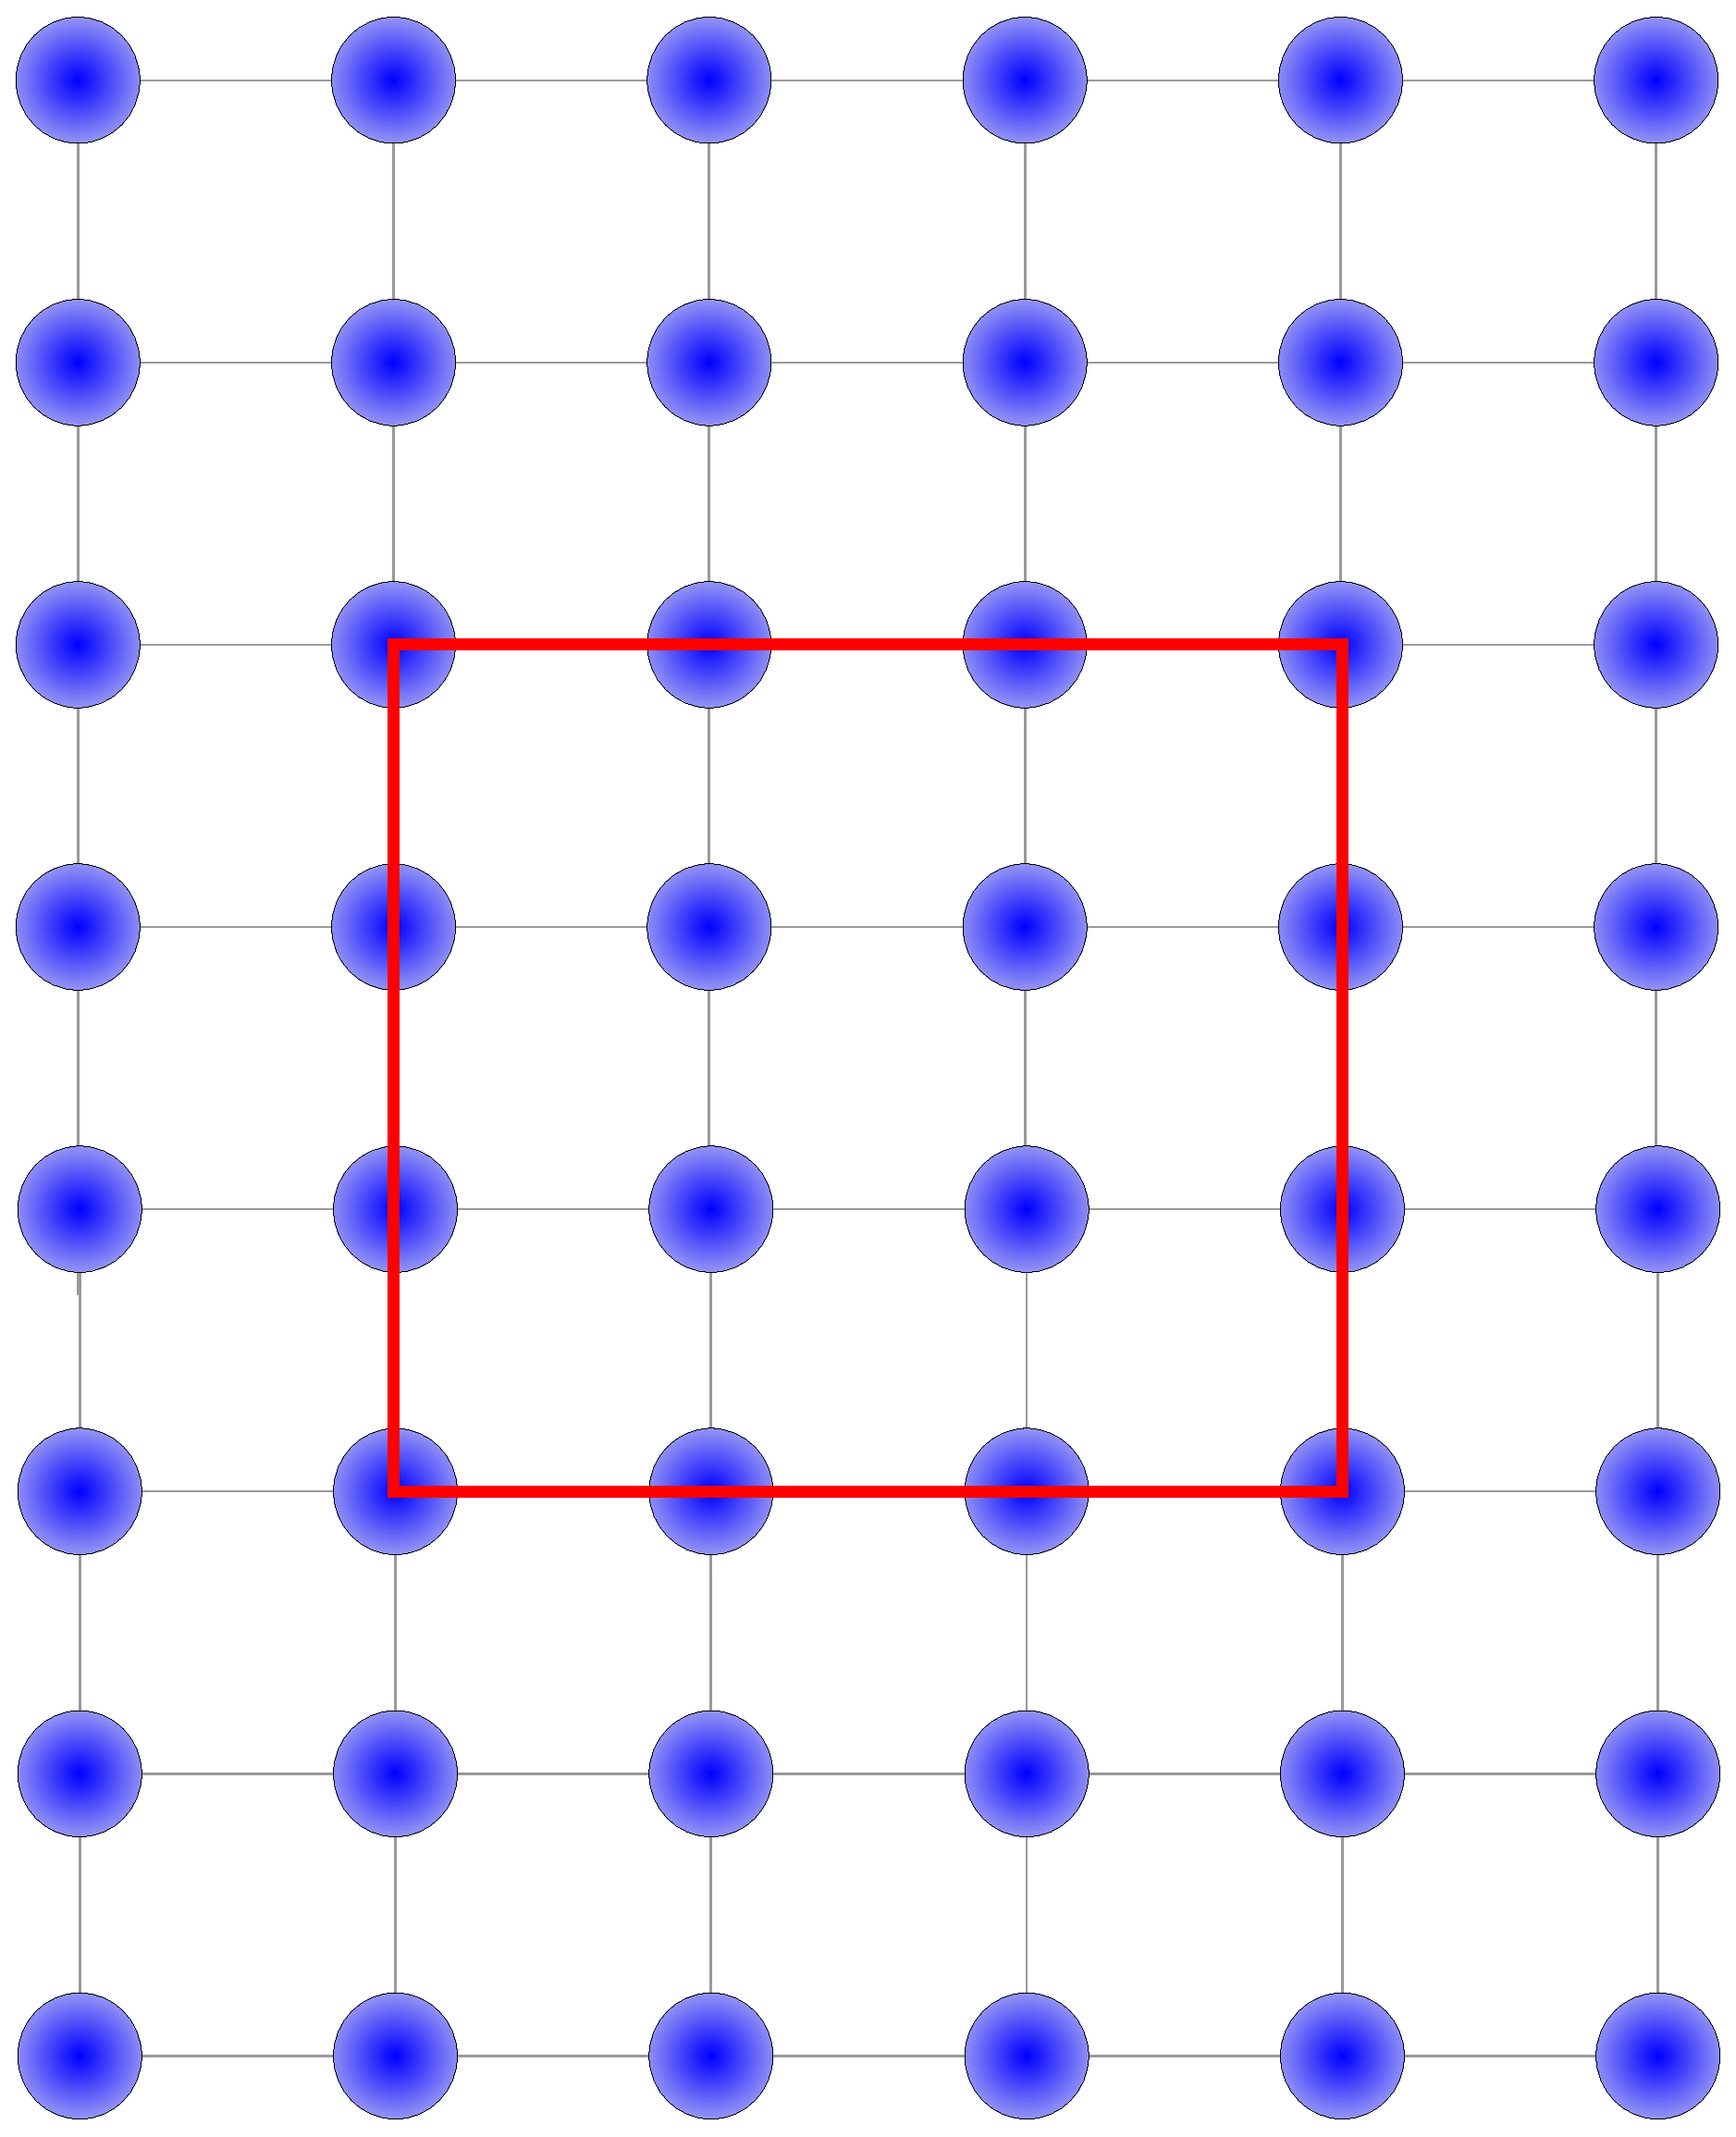
\includegraphics[height=2.5in]{Perfect_crystal_loop}
\caption{A perfect crystal with a complete circuit shown in red.}
\end{subfigure}
\begin{subfigure}{0.4\textwidth}
\centering
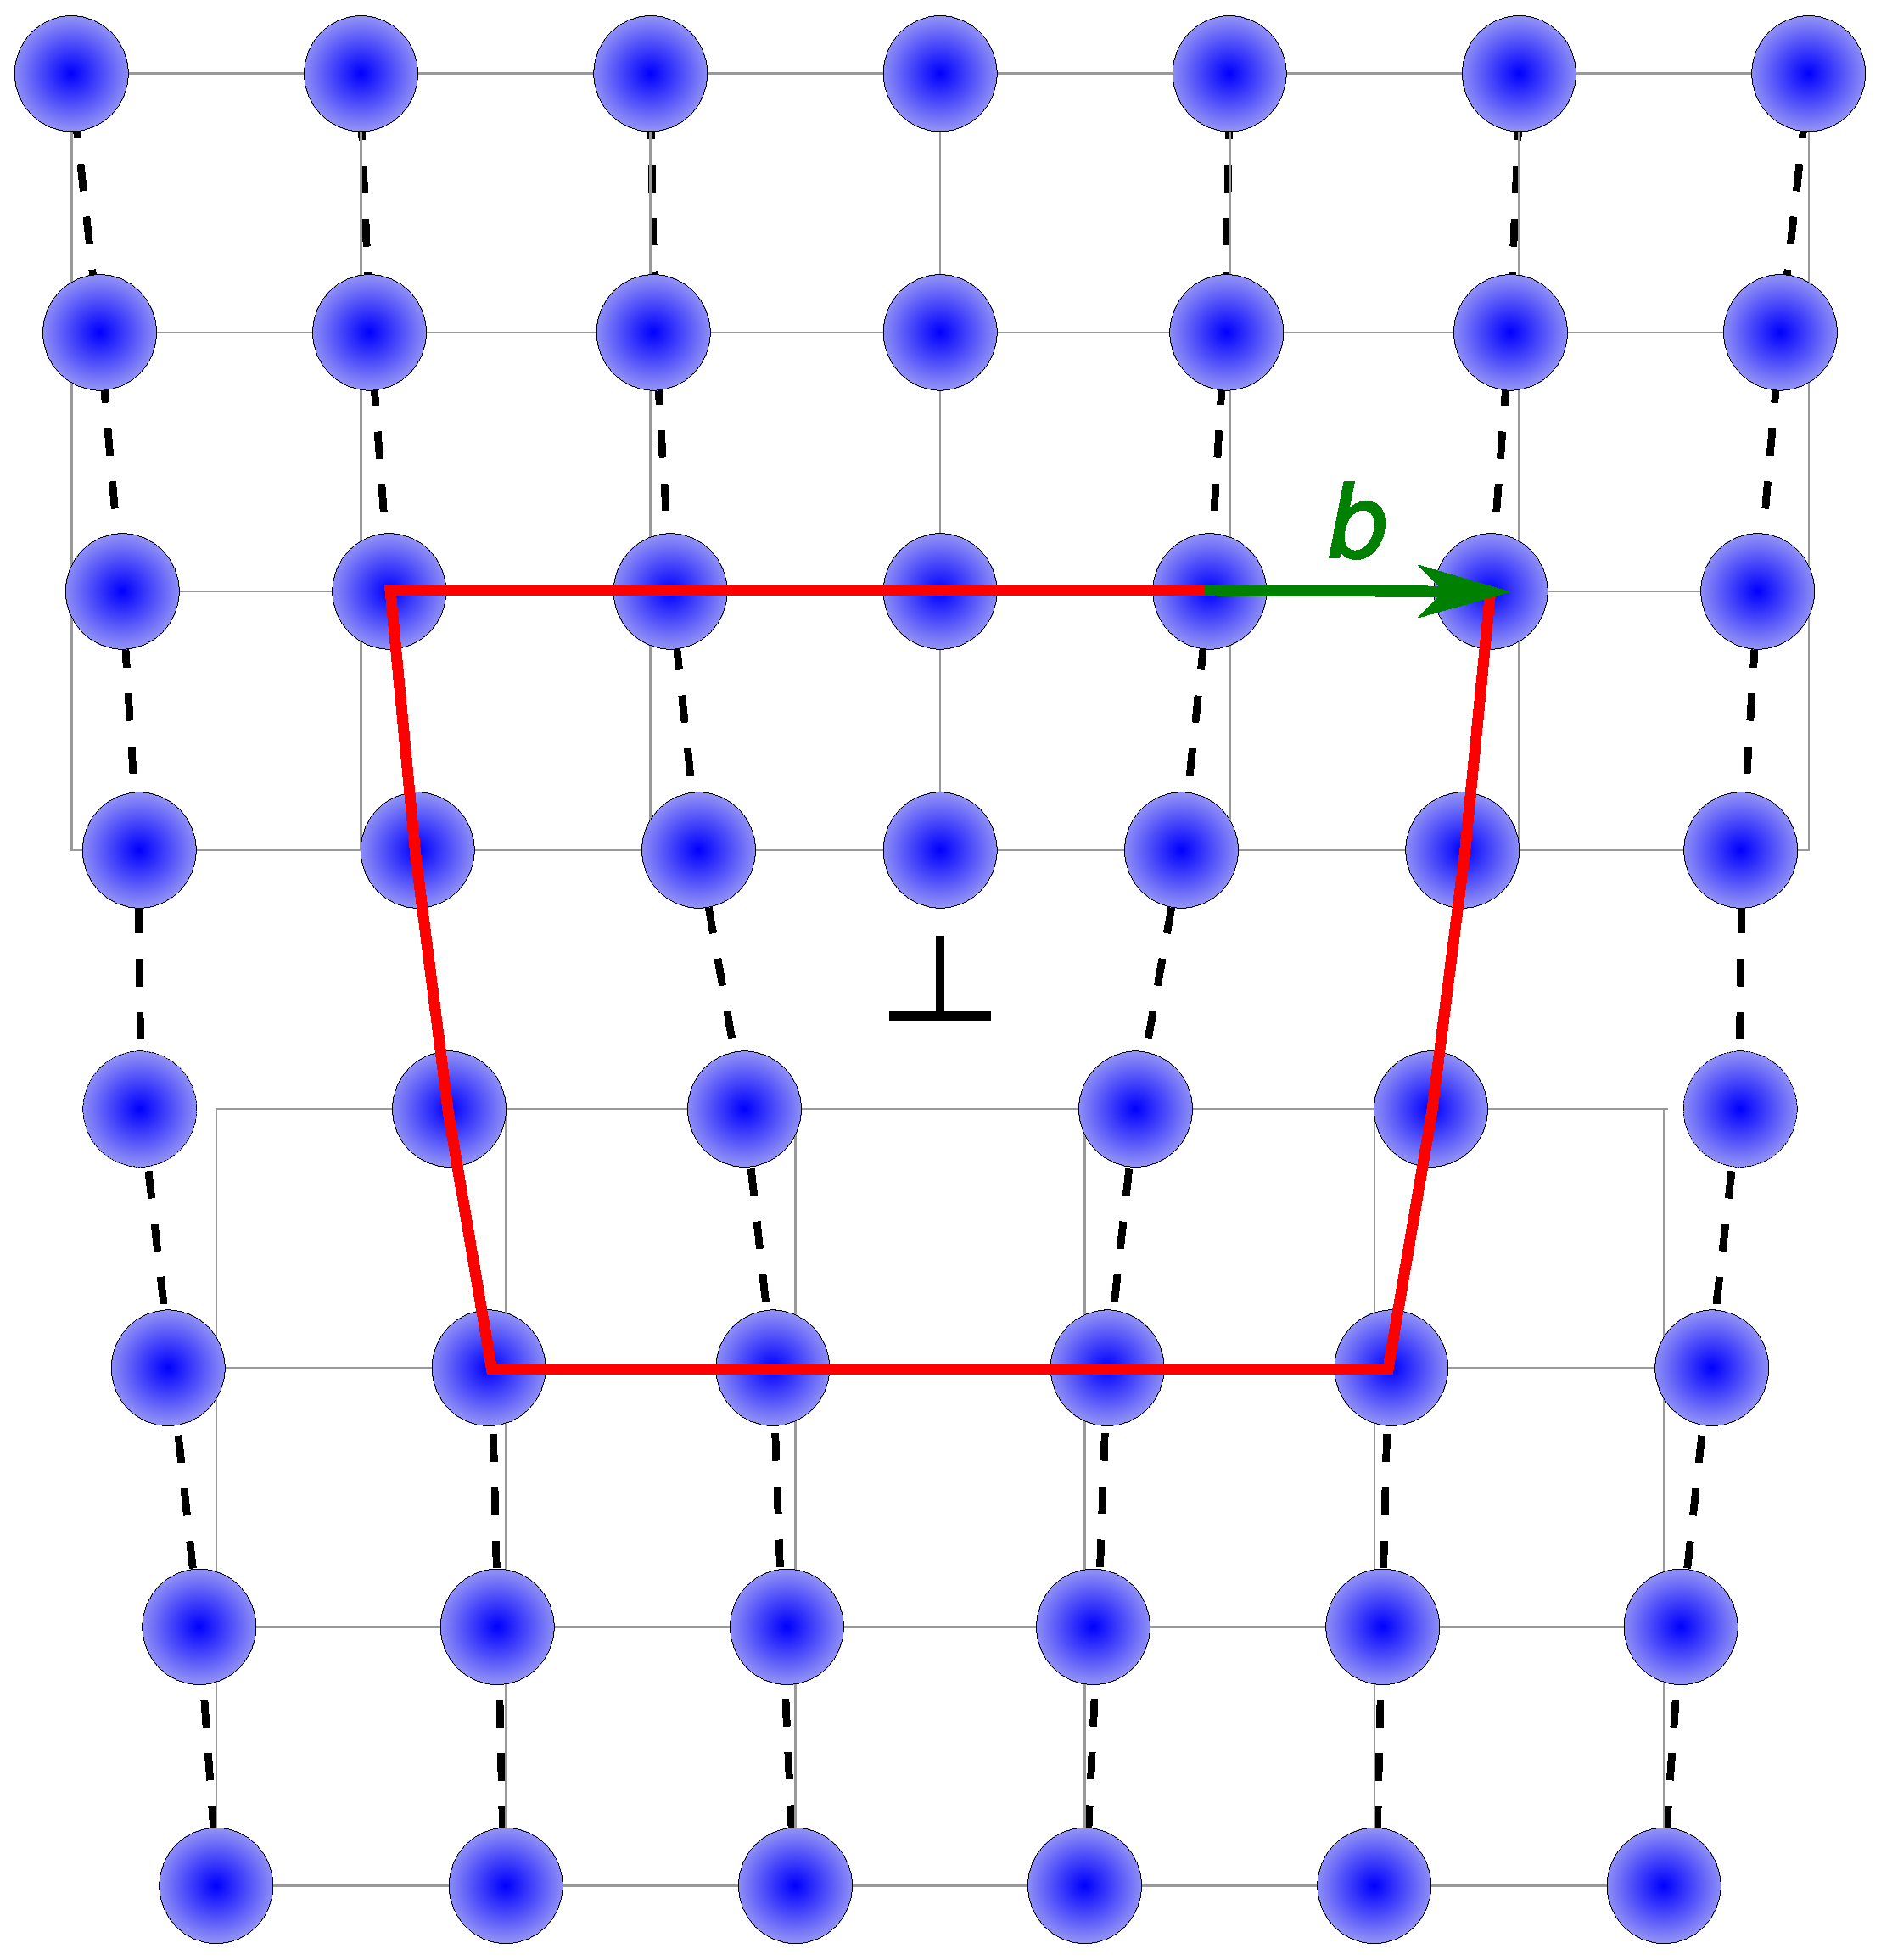
\includegraphics[height=2.5in]{Edge_Dislocation_loop}
\caption{An edge dislocation with an incomplete circuit. \label{fig:Edge_disloc_loop}}
\end{subfigure}

\caption{Inserting a half plane of atoms which terminate in a dislocation and a Burgers circuit to show the Burgers vector. \label{fig:burgers_loops}}

\end{figure}

\begin{figure}
\centering
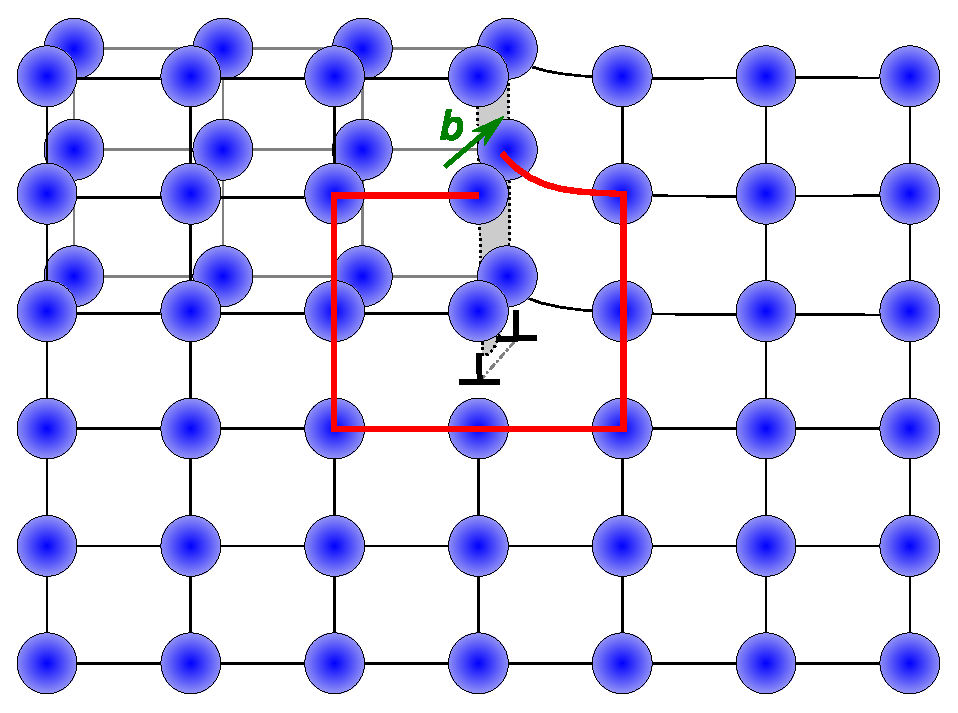
\includegraphics[width=0.7\textwidth]{screw_disloc_loop}
\caption{Schematic of a screw dislocation with a Burgers loop formed in a similar way to \autoref{fig:burgers_loops}. The displacement is parallel to the dislocation line in contrast with edge dislocations. \label{fig:screw_disloc}}
\end{figure}




Dislocations can be described in terms of a slip direction, a line direction and a slip plane. The slip direction is simply the direction parallel to the Burgers vector, this is the relative displacement caused by the passage of a dislocation through a region of crystal. The identification of the Burgers vector is done with a Burgers loop, a loop comprised of steps between nearest neighbours is defined that would be closed in a perfect crystal is defined. The same set of steps is undertaken in a dislocated crystal and the loop is no longer closed and the displacement vector between the endpoints is the Burgers vector. This is shown for an edge dislocation in \autoref{fig:burgers_loops}, where the Burgers vector is perpendicular to the line vector, and a screw dislocation in \autoref{fig:screw_disloc}, where the Burgers vector is parallel to the line vector. The line direction can and does vary along the length of the dislocation but is simply the line defined by the defective region of crystal. The slip plane is the crystallographic plane in which the dislocation can move and must contain the slip direction and line direction; where the line and the slip directions are not parallel the slip plane is defined by these two vectors, but for screw dislocations which have the slip direction and line directions parallel the plane is not so constrained, instead the possible slip planes are those that allow easy movement, i.e. lower forces or smaller energy changes, and depending on the crystal symmetry there may be several. This allows screw dislocations to change the plane they are moving in, a process known as cross slip \cite{Hirth_Lothe1982intro}.

Real dislocations are not neat and instead of lining up with convenient crystallographic axes will curve and bend. This usually gives rise to a mixed and varying character of dislocation with the Burgers vector neither parallel nor perpendicular to the line vector. These mixed dislocations are usually described as the sum of edge and screw components.

There are conventions about the sign of dislocations, taking line vectors into or out of the page and defining the sense of Burgers loops and the Burgers vector defined from the finish to the start etc. Given that the symmetry of most of the crystals of interest is high enough to ensure that all these choices are usually arbitrary the only thing that will be highlighted here is that if the sense of a dislocation is reversed then its stress/strain field will reverse in sign. Hence oppositely signed dislocations attract to lower the stored elastic energy and potentially to annihilate line length, while like-signed dislocations will repel to lower the elastic stored energy.



\FloatBarrier

\subsection{Historical overview}
In the early twentieth century there were many observations of real world materials strengths that could not be reconciled with the theoretical shearing strength of a perfect plane of atoms. Indeed for a long time this was neglected because, as \citet{gordon1991} puts it:
\begin{quote}
``Until about 1934 the Establishment explanation of these phenomena was remarkably unconvincing and seems to have reflected mainly a desire not to be asked embarrassing questions.''
\end{quote}

In 1934 the edge dislocation was proposed by \citet{orowan1934i,orowan1934ii,orowan1934iii}, \citet{Taylor1934}, and \citet{polanyi1934} to explain the discrepancy between the ideal strength of crystal and the observed strengths of real materials. It was around this time that work undertaken by \citet{Volterra1907} and others %% Cite some here
on elastic behaviour of homogeneous isotropic continua was related to plastic flow of crystalline materials and indeed idealised dislocations in elastic continua are termed Volterra dislocations. By the end of the decade \citet{burgers1939} had described screw dislocations.

It was not until the 1950s that experimental evidence for the existence of dislocations was produced ; the principle evidence at that time being growth surfaces of single crystals, preferential etching of a crystalline material at dislocations and x-ray studies of arrays of dislocations in the bulk \cite{Forty1954}. 

Growth surfaces provide evidence for dislocations because, as \citet{Frank1949} predicted in 1949, a step could terminate by the intersection of a dislocation with a free surface, or conversely a dislocation intersecting with a free surface would necessarily create a step. The observation of such steps was very soon after Frank's prediction in 1950 by \citet{Griffin1950}.

Etch pits were shown to form at the intersections between dislocations and free surfaces by \citet{Horn1952} who observed that the configuration of etch pits matched the pre-existing surface growth features that arise from screw dislocations.

Arrays of dislocations can be detected by x-ray methods. The observation of Laue spots of an single crystal through the processes of plastic deformation and what we now call recovery provided indirect evidence for the existence of dislocation arrays. The process, described by \citet{Cottrell1949}, is as follows: Initially sharp Laue spots exist for a relatively perfect single crystal. These spots are then smeared during the process of plastic deformation which creates large numbers of dislocations throughout the crystal. The spots then split into distinct sharp spots during the process of recovery by which annealing allows dislocations to align into arrays and thereby minimise the elastic strain energy. These arrays form sub-grains, regions of perfect (or at least relatively perfect) crystal separated by low angle boundaries formed by arrays of dislocations.


\subsection{The stress required to move a dislocation}

Though mathematical descriptions of dislocations in isotropic elastic continua date back to 1907 \cite{Volterra1907} the energies and forces around dislocations in crystalline lattices and the  was not considered until much later. In 1940 \citet{Dehlinger1940} and \citet{Peierls1940}. The former presented the application of the Frenkel-Kontorova model, a one dimensional array of balls connected by springs on a periodic potential/substrate, to approximate a dislocation.

The latter, Rudolph Peierls, was one of the physicists working during the great advent of quantum mechanics and most of his work was in that field, he was lectured by Planck, he worked with Pauli, Landau and others and
notably developed the idea of zones in the physics of phonons before Léon Brillouin and the statistical mechanics of alloys which formed the basis of mean-field theories for structural phase changes.
However during his education he received a grounding in classical physics at Arnold Sommerfeld's lectures in Munich and so it was that he was suitably equipped when presented with the problem of dislocation motion by Egon Orowan; as Peierls remarked he knew nothing about dislocation but he did know classical elasticity \cite{Edwards1996}.


Peierls presented the first formal solution for the dislocation displacement potential in a rather short note \cite{Peierls1940} and the idea was extended by \citet{Nabarro1947}. The model is remarkably simple; consider two semi-infinite perfect crystals with their lattice aligned but some initial misalignment between them as shown in \autoref{fig:semi_infinite_crystals}. We can join them along what will become the slip plane. An edge dislocation is formed where the energy of the system is lowered by displacing atoms from their initial positions to localise the misalignments around the dislocation core, usually taken to be the origin. I.e. when the energy of a planar defect is higher than that of the linear defect and dislocation will form.


\begin{figure}
\centering

    \begin{subfigure}{0.4\textwidth}
        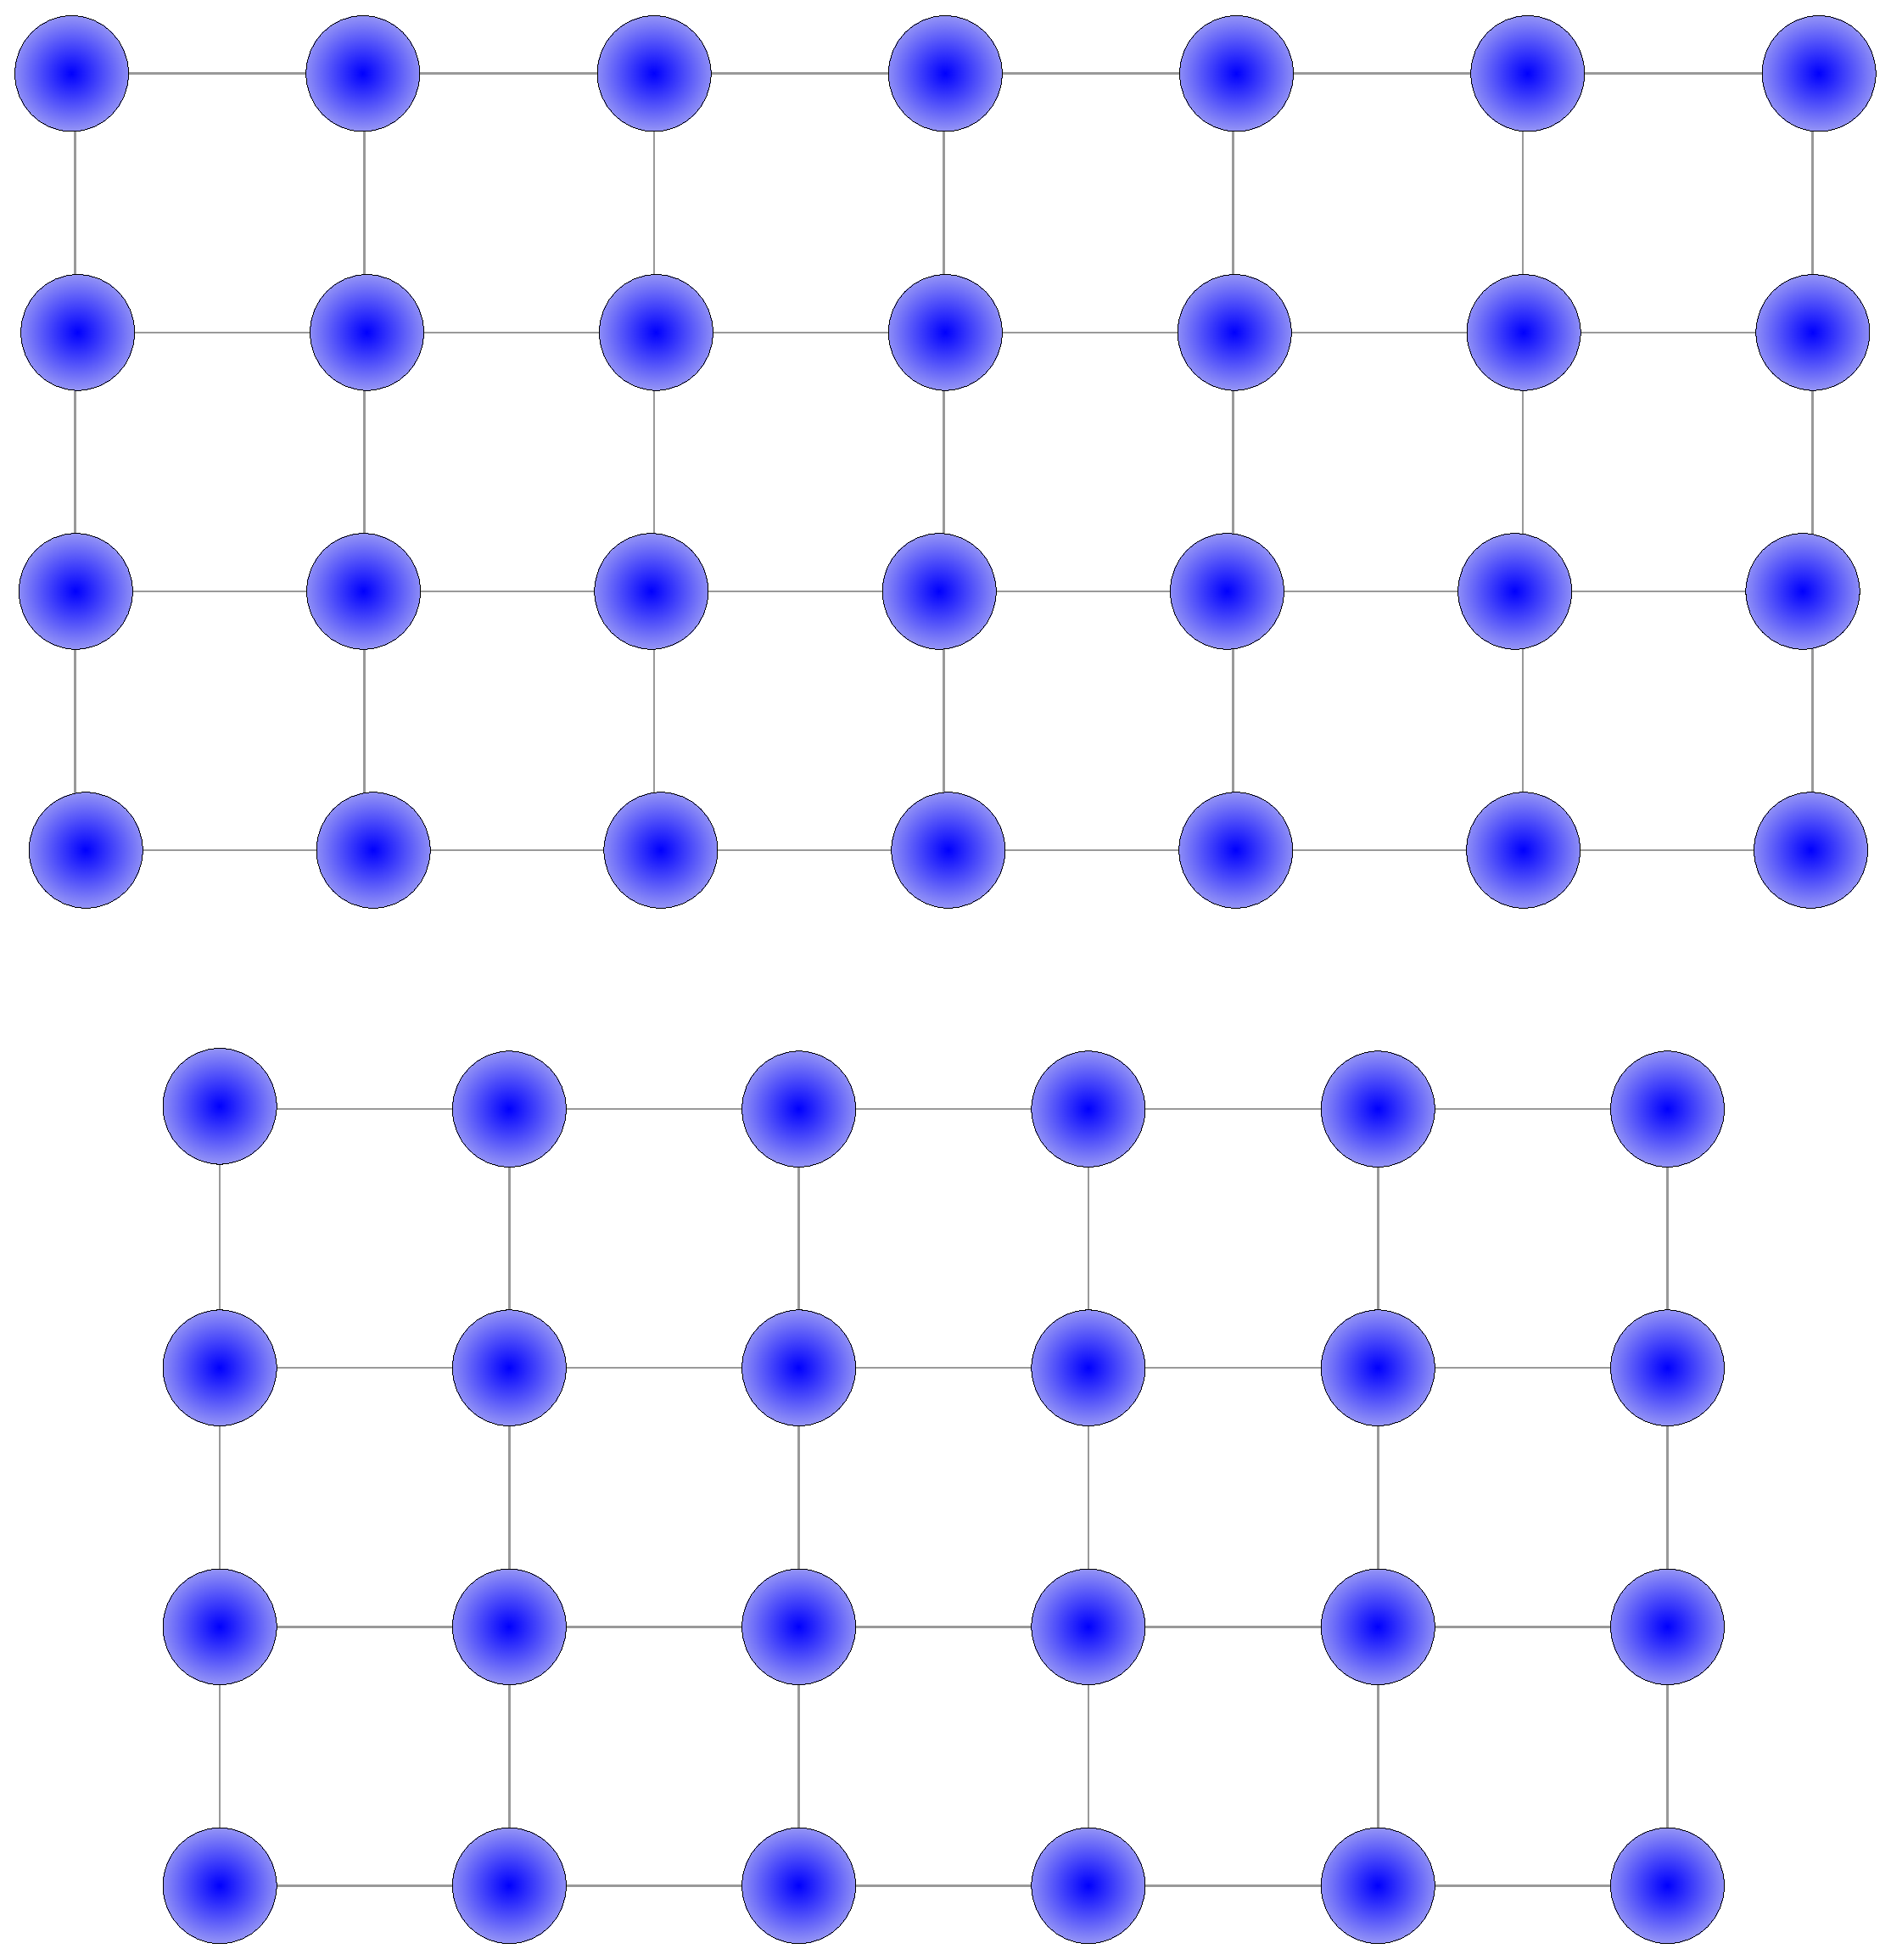
\includegraphics[width=\textwidth]{Half_crystals}
        \caption{Two semi-infinite crystals \label{fig:semi_infinite_crystals}}
    \end{subfigure}

    \begin{subfigure}{0.4\textwidth}
        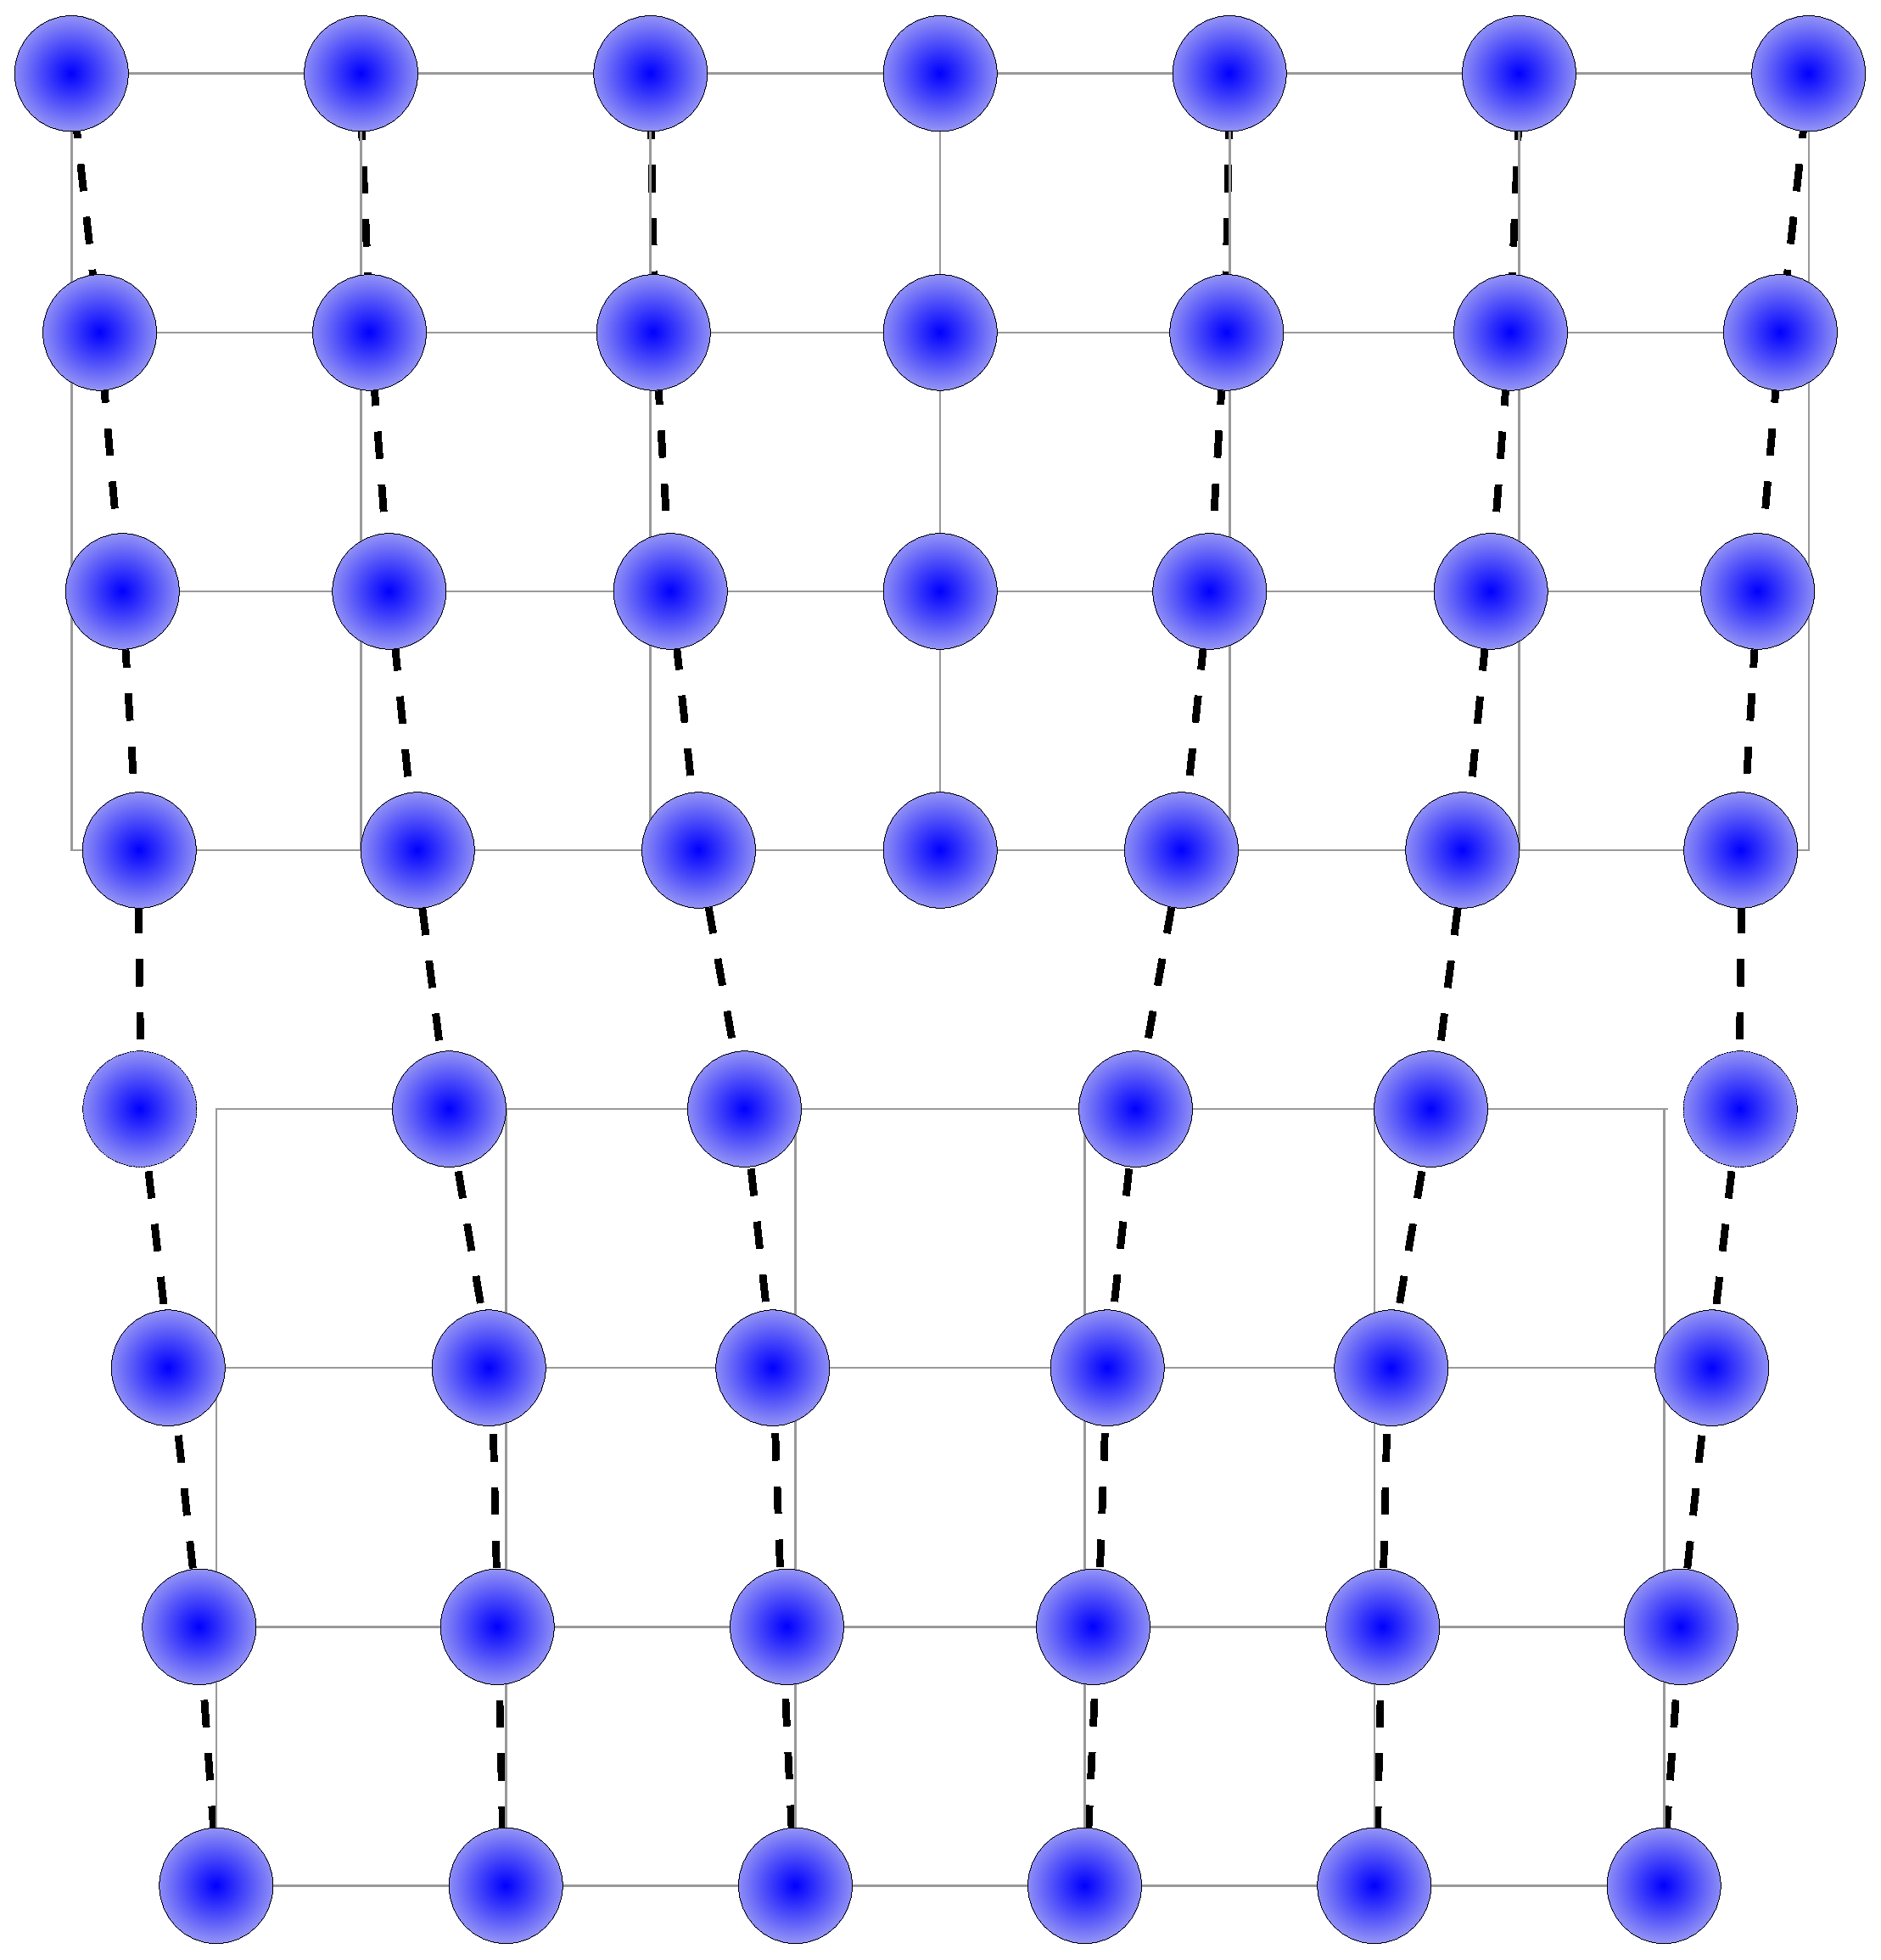
\includegraphics[width=\textwidth]{Edge_Dislocation}
        \caption{A schematic edge dislocation\label{fig:joined_half_crystals}}
    \end{subfigure}

    \caption{Schematics showing the creation of an edge dislocation in a simple square lattice by the joining of two misaligned half crystals. \label{fig:edge_disloc}}
\end{figure}



The Peierls model then estimates the energy of the configuration by considering two restoring forces generated by the atomic arrangement. Firstly the bonds parallel the slip plane will be either extended or contracted, for example the bond between atom $A$ and $B$ has been contracted by the amount $\delta$, this will tend to oppose the concentration of misalignments to the core and  is zero in the case of no displacements from the initial positions, Peierls assumed this to be a constant energy found from the linear elastic stress field of a Volterra dislocation. Secondly the misalignment of bonds across the slip plane, the bond between atom $B$ and $C$ is misaligned by a lateral distance of $\phi$. This misalignment energy will tend to favour the concentration of the misalignments to the core and is a maximum in the case of no displacement from the initial position.

The energy change is then calculated for different displacements from the symmetry position shown in \autoref{fig:edge_disloc}. This displacement is usually parametrised by the term $\alpha$ which is taken to be zero at the initial symmetrical position and increase to one after a displacement of $b$ to the next symmetrical position. 






The energy of the dislocation is the sum of all these contributions. This gives rise to a size, or width, of a dislocation. The width of the dislocation is defined as the distance from the core at which the misalignment across the slip plane is half its maximum. Peierls calculated this for an isotropic elastic solid and accounting for only the atomic planes immediately adjacent to the slip plane and found it to be 

\begin{equation}
w = \frac{d}{1-\nu}
\label{eqn:width_isotropic}
\end{equation}
where $d$ is the plane spacing across the slip plane and $\nu$ is the Poisson ratio.


Peierls gave the critical stress, now usually termed the Peierls Stress, for an isotropic elastic material, in terms of the ideal shear strength as calculated for uniform slip, as


\begin{equation}
\frac{\tau_p}{\tau_{ideal}} = \frac{4 \pi}{1 - \nu} (5.8 - \log|1-\nu|) \exp\left(-\frac{4\pi}{1 - \nu}\right).
\end{equation}

This was refined by \citet{Nabarro1947} and the direct summation of the discrete contributions was developed by Cottrell and Nabarro \cite{cottrell1953dislocations}. The result of that summation is



\begin{equation}
\tau_p = \frac{2\mu}{1-\nu} \exp\left( - \frac{4\pi w}{b} \right)
\end{equation}
where $\mu$ is the shear modulus and $b$ is the burgers vector.

For an isotropic material the width can be substituted from \autoref{eqn:width_isotropic}:

\begin{equation}
\tau_p = \frac{2\mu}{1-\nu} \exp\left( - \frac{2\pi d}{(1-\nu)b} \right).
\end{equation}

Although a simple model based on fairly large assumptions the method moved dislocation theory on in two ways: firstly continuum elasticity could not account for energy changes as the dislocation moves, this is the small difference between the continuous integral and discrete sum that depends on the core position, and secondly this approach removes the singularity at the core predicted by continuum elasticity for Volterra dislocations.


An important point to note here is that the Peierls stress is extremely sensitive to the size of the dislocation, $w$, and therefore to the factors that control the width; in the case of isotropic materials the model is explicitly sensitive to the lattice geometry defined by $d/b$ and the Poisson ratio, $\nu$.



Peierls found the perhaps surprising result that the energy changes have a periodicity of $b/2$ rather than $b$, this has been ascribed to the summation procedure of the energy of the misaligned bonds across the slip plane, of which there has been much discussion \cite{Hirth_Lothe1982lattice_periodicity,Lu2000peierls}, Peierls summed over the atoms above the slip plane and below the slip plane independently, the ``double-counting'' scheme, later models used a ``single-counting' scheme in which the assumption of small displacements is dropped and the misalignment of an atom above the slip plane is dependent on the final position of the atoms below the slip plane. This is given as the reason the Peierls barrier had a wavelength of $b/2$ rather than $b$ \cite{Hirth_Lothe1982lattice_periodicity,Lu2000peierls} though it has been suggested that the problem is an artefact that arises from an assumption of small displacements and that using the final rather than initial positions of the atomic rows resolves the difficulties \cite{Huntington1955}. As will be discussed below there is another possible explanation for the change in period that depends on the exact formulation of the energy calculations and whether the $\alpha=1/2$ position is symmetrically equivalent to the $\alpha = 0, 1$ positions. The periodicity of $b/2$ is easily explained on this basis because Peierls assumed that both the elastic energy and the dislocation geometry remained constant and the only changes in the energy were therefore based on misaligned bonds across the slip plane. These assumptions produce an atomic configuration at $\alpha=1/2$ that is the mirror through the slip plane of the $\alpha=0$ configuration, which must give the same energy since the misalignment potential used by Peierls is symmetrical.




There have been many criticisms of and modifications to the Peierls model in the years since but these have largely focused on adjusting the assumptions of the original method.
In 1951 \citet{Foreman1951} introduced phenomenological potentials to describe the energy of the misaligned interactions across the slip plane, they discovered that the width of the dislocation was predicted to be larger than that of the original treatment and was coupled with a decrease in the Peierls stress. .
In 1955 \citet{Huntington1955} modified the model to double the periodicity and so account for crystals in which a displacement of half a burgers vector is not symmetrical with no displacement, or in other words broke the mirror symmetry of the slip plane. 
\citet{Maradudin1959} considered a completely atomistic three dimensional model of a screw dislocation but did not consider radial displacements. That work only evaluated the energies of the symmetric and anti-symmetric configurations and so only estimated the energy change, not the maximum stress.



In 1994 a fully discrete model was developed by \citet{Ohsawa1994}. This model made similar assumption to the original Peierls model in that the only energy changes were in the sheared misaligned bonds across the slip plane but instead of solving for an analytical solution Ohsawa et al directly summed the energy of an atomic configuration that included 84 atoms, or 21 atomic spacing either side of the dislocation core. The model made no assumptions about the displacement field and instead iteratively improved all the atomic positions to find the equilibrium configuration. This was done for increasing applied external stresses until there was no stable configuration, i.e. slip would occur.



\citet{Bulatov1997} incorporated the concept of generalised stacking fault (GSF) energies into the Peierls model and successfully applied it to real systems \cite{Lu2000aluminium}. This addresses a fault in the original Peierls formulation that the sinusoidal potential used to calculate the misalignment energy is too high and steep. \citet{Ohsawa1994} had already attempted to address this by using alternative potentials, but they were essentially arbitrary functions that fitted the shear modulus at small strains Instead Bulatov et al retained the variational approach but used density functional theory (DFT) calculations to generate a misalignment potential. They extended this to provide a three dimensional potential to allow both lateral and vertical displacements of the atoms in the slip plane. This is important around the core where large strains mean that the energy contributions are very inaccurate, and so by using the DFT to calculate a misalignment potential the Peierls model can bridge the length scales between the large scale stress and strain fields around the dislocation and the large local displacements at the core. This is no longer analytically solvable but is not difficult to solve numerically, the only limit being computational time.

Analytical approaches have continued, \citet{Joos1997} developed a closed form solution that was valid for narrow dislocations, where as the original model relied on the assumption of a wide dislocation for simplicity, and achieved a significantly better agreement with experiment than the original formulation. The model proposed by Joós and Duesbery required input parameters calculated by empirical or ab initio methods but used these as parameters of a closed form solution, in particular they required the maximum restoring stress for the glide plane, i.e. the maximum gradient of the GSF energy.

\begin{figure}
\centering
\begin{subfigure}{0.4\textwidth}
\centering
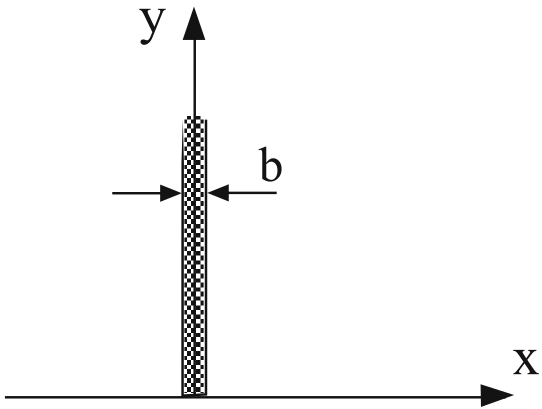
\includegraphics[width=0.75\linewidth]{Dislocation_with_discontinuity}
\caption{Volterra dislocation.\label{fig:disloc_discontinuity}}
\end{subfigure}%
\begin{subfigure}{0.4\textwidth}
\centering
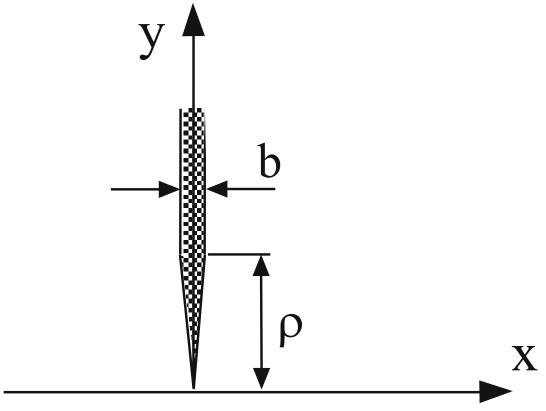
\includegraphics[width=0.75\linewidth]{Dislocation_without_discontinuity}
\caption{Lubarda dislocation\label{fig:disloc_no_discontinuity}}
\end{subfigure}
\caption{The displacement discontinuities in the traditional Volterra dislocation and that used by Lubarda and Markenscoff that removes the singularity at the core. From \cite{Lubarda2007}\label{fig:discontinuity}}
\end{figure}

A continuum elasticity solution was presented by \citet{Lubarda2007} which removed some of the limiting assumption of the original Peierls model, notably the assumption of fixed dislocation geometry as the dislocation was translated from one symmetrical position to the next and that only the misfit energy of the slip plane changes and that the elastic energy away from the slip plane remains constant. The main challenge to using continuum elasticity to solve the Peierls model directly is the singularity in stress and strain at the dislocation core. 
This singularity arises where the displacement discontinuity of a Volterra dislocation across the half plane of an edge dislocation terminates at the core shown in \autoref{fig:disloc_discontinuity}. 
By introducing a gradual increase in the displacement discontinuity across the plane of an edge dislocation from zero at the core to $b$ at some finite distance, as shown in \ref{fig:disloc_no_discontinuity}, Lubarda and Markenscoff were able to formulate a tractable linear elastic continuum problem which produced much better agreement than previous analytical solutions. They found this distance to be be interpretable as the width of the dislocation giving rise to displacements that are consistent with the original Peierls model. 



In 2006 \citet{Clegg2006} used an atomistic approach to the strains outside of the slip plane in addition to the energy of the misalignment across the slip plane. The atomic displacements were taken to have the same form as Peierls had derived, that is

\begin{equation}
u(x_0) = \pm \tan^{-1}\frac{x_0}{w}.
\end{equation}

where $x_0$ is the initial coordinate in the dimension parallel to the burgers vector and $w$ is the dislocation width, now a parameter to be optimised with no closed form solution. The misalignment energy was taken to be

\begin{equation}
U^{x} = \frac{Gb^3}{4\pi^2 d} \sum_n \left[ 1 - \cos \left(\frac{2\pi \phi_n}{d} \right)\right]
\end{equation}
 
 and the in-plane strain energy was taken to be 
 
 \begin{equation}
 U^i = \frac{E}{2(1-\nu^2)} (b\cdot d) \sum_n \epsilon_n^2
 \end{equation}

where $G$ is the shear modulus of the material, $E$ is the Young's modulus, $\nu$ is the Poisson ratio, $b$ is the Burgers vector, $d$ is the slip plane spacing, $\epsilon$ is the strain and is calculated by $\epsilon = \delta/b$, $\delta$ is the extension of an in plane bond and $\phi$ is the misalignment of the bond across the slip plane. $\phi$ and $\delta$ are shown in \autoref{fig:detail_of_peierls}. The energies are then summed over interaction between atomic rows extending 1000 atomic spacings either side of the dislocation core.

The width no longer has an analytical solution so must be found numerically. The variation of the energy was shown to be smooth and have only one minimum because the misalignment energy is monotonically increasing with increasing width and the elastic in plane strain energy is monotonically decreasing.

It is interesting to note that this formulation restores the symmetry that is destroyed in the calculation of elastic energy by continuum elasticity in that the strains above and below the slip plane are symmetric. So despite allowing the strain energy to vary as the dislocation moves this model has the same period as the original Peierls model of $b/2$.

\begin{figure}
\centering
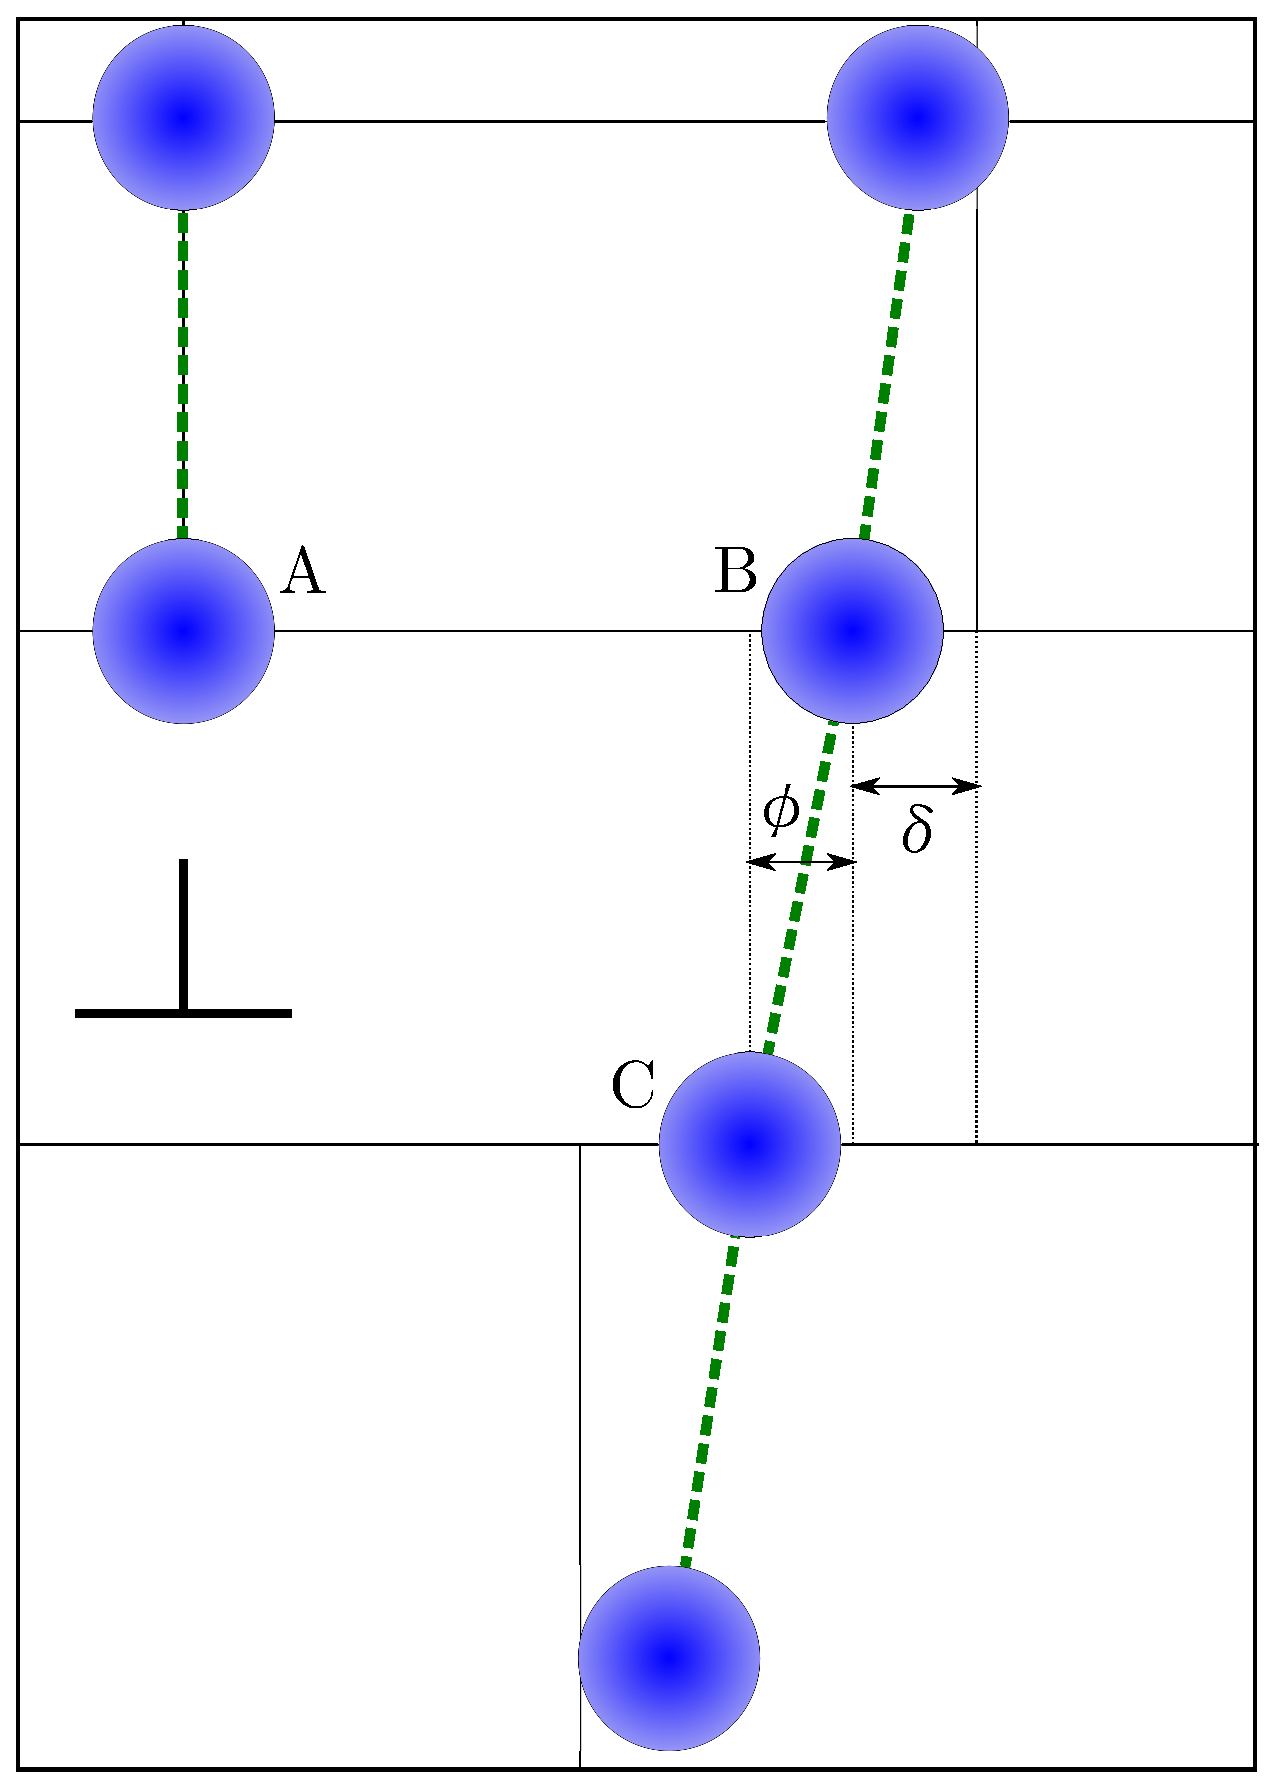
\includegraphics[width=0.6\textwidth]{peierls_model_detail}

\caption{Detail of the local displacements around the dislocation core. $\delta$ is the extension of the bond paralell to the slip plane between atoms A and B, while $\phi$ is the misalignment of the bond across the slip plane between B and C.\label{fig:detail_of_peierls}}
\end{figure}




\newpage

\subsection{Ductility criteria}
\label{subsec:ductility_criteria}
 In most structural applications a catastrophic brittle failure by fast fracture is unacceptable, so there is great interest in the failure mode of materials. Additionally many materials used in devices or coatings both protective and functional often fail by brittle fracture and so a material that is more ductile, at least relatively, has the potential to greatly extend the lifetime of these materials and components.
There have been a number of attempts to find ductility criteria to predict from simple and easily measurable properties whether a material will fail in a ductile or a brittle manner.
The Pugh ratio, $B/G$, is one of the most widely known and is still used today. Defined as the quotient of bulk modulus over the shear modulus, it is used to indicate the relative ease of either plastic deformation or brittle fracture. High values of this ratio should tend to indicate ductility while low values indicate brittleness. This can be physically justified on the basis that the ease of slip is proportional to the shear modulus, as discussed above the Peierls model finds the Peierls stress to be $\tau_p = 2G / (1-\nu) \exp[-2d/(b(1-\nu))]$ so for a given lattice, i.e. constant $d/b$, the shear flow stress should scale with the shear modulus; in a similar way the ease of fracture must be related to the ease of separating layers of atoms which must depend on the stiffness and the surface energy and the bulk modulus is a reasonable proxy for these and gave good results empirically when \citet{Pugh1954} analysed a wide range of material data.

However this does not accurately capture reality. For example two face-centred cubic metals, aluminium and copper, $B/G$ of 2.74 and 3.00 respectively. These metals both show large elongations to failure while Rhodium and Iridium, $B/G$ of 1.77 and 1.74 respectively, show small elongations to failure \cite{Pugh1954}. However very brittle phases are easily found with similar values of $B/G$, the C15 Laves phases \cite{Stein2004,Stein2005} \ce{NbCr2} and \ce{HfV2} also have large values of $B/G$, 2.88 and 3.47 respectively \cite{Chu1995}, but exhibit no significant plasticity whatsoever. In contrast \ce{Ti3SiC2} has a value of $B/G$ of 1.37 \cite{Barsoum2011} but shows very easy slip.



%%%%%%%%%%%%%%%%%%%%%%%%%%%%%%%%%%%%%%%%%%%%%%%%%%%%%%%%%%%%%%%%%%%%%%%%%%%%%%%%%%%%%%%%%%%%%%%
% Maybe the graph of $B/G$ ratios for fcc metals and Laves phase here
%%%%%%%%%%%%%%%%%%%%%%%%%%%%%%%%%%%%%%%%%%%%%%%%%%%%%%%%%%%%%%%%%%%%%%%%%%%%%%%%%%%%%%%%%%%%%%%



\citet{rice1974} suggested an alternative with rather more theoretical backing based on the energetics of sharp crack tips and whether blunting dislocations can be spontaneously emitted. The analysis used the Peierls approach to evaluate the energy of the dislocation close to free surfaces and found that the term $Gb/\gamma_s$, where $\gamma_s$ is the surface energy, $G$ is the shear modulus and $b$ is the Burgers vector, should be a dimensionless value that in some way reflects the propensity to fail by either ductile or brittle means and is justified along similar lines in that $Gb$ will scale with the energy of emitting a blunting dislocation, high values will oppose the formation of dislocations and blunting of cracks, thus favouring brittle failure; $\gamma_s$ represents the energy of the crack and high values will tend to favour reduction of the surface by blunting and favour ductile failure. The criterion was updated by \citet{Rice1992} to be the quotient $\gamma_{us}/ \gamma_s$ where $\gamma_{us}$ is the unstable stacking fault energy and $\gamma_s$ is still the surface energy but follows essentially the same reasoning but no longer makes the assumption that $\gamma_{us}$ scales linearly with $G$.

An alternative condition was put forward by \citet{Zhou1994} that does not include the surface energy. They propose the energy to blunt a crack by dislocation emission is dependent on $\gamma_s$ in the same way as the energy of growing the sharp crack since the formation of a dislocation creates ledges and alters the surface area. In this way the ratio of the energies is independent of the surface energy (though the absolute value of either energy is clearly dependent on $\gamma_s$) and so the crossover from brittle to ductile behaviour is also independent of the surface energy. They find instead that the appropriate quotient is $\gamma_{us} / Gb$ and set a critical value of 0.014. As the authors note this is an interesting result because the critical threshold is not the cross over in a competition between two processes, one of fracture and one of plasticity, but instead is equivalent to a critical value of the Peierls energy.

One draw back of these more physically insightful approaches is that strictly they apply only for one slip system and one mode of fracture on one plane and so should be applied for all possible combinations with some appropriate statistical weighting. Given that experimental determination of the unstable stacking fault energy and the surface energy is laborious and calculations quickly become time consuming as combinations of fracture and slip modes are considered these criteria can become rather cumbersome. They also rely in all cases on the assumption that firstly the energy barrier for slip, the Peierls energy, scales with the stacking fault energy or shear modulus and secondly that the stress required for slip scales simply with the Peierls energy. These quantities will clearly be linked but it is unlikely that the relationships are as simple as would be needed for such ductility criteria to be reliable.

For example the phases titanium carbide, \ce{TiC}, and the ternary carbide \ce{Ti3SiC2}. The above models all correctly predict that \ce{TiC} is brittle, the value of $\gamma_s / \gamma_{us} = 1.76$ is too small with values in excess of 3 required for ductility \cite{Price1992,Yu2003} and the values of $Gb/\gamma_s = 20.48$ and $\gamma_{us} / Gb = 0.032$ being far to large to indicate ductile behaviour \cite{Yu2003,Medvedeva2011}. However these same criteria take similar values for \ce{Ti3SiC2} for which $\gamma_s / \gamma_{us} = 1.42$, $Gb/\gamma_s = 27.3$ and $\gamma_{us} / Gb = 0.0219$ \cite{Medvedeva2011,Farle2015}. The Pugh model and the two Rice models \cite{Pugh1954,rice1974,Rice1992} actually predict the MAX phase to be more brittle than stoichiometric titanium carbide. This is clearly is at odds with reality since titanium carbide has a yield stress of over \SI{2}{\giga\pascal} at temperatures below \SI{600}{\celsius} \cite{Miracle1983} while at room temperature the critical resolved shear strength of \ce{Ti3SiC2} is reported to be \SI{36}{\mega\pascal} \cite{Barsoum1999}, though reanalysis of the data has this somewhat higher at \SI{77}{\mega\pascal} \cite{Humphrey2012}.


The inability to capture or predict the ductility or brittleness of materials limits the use of these ductility criteria, so that while they highlight some eprhaps noteworthy trends they could not have been used to predict the anomalous yielding in the MAX phases and other layered compounds that are now being commercialised to take advantage of the high temperature capability that arises from their chemistry, as a stoichiometric compound that can include \ce{Si} or \ce{Al} MAX phases are corrosion resistant and stable to high temperatures \cite{Radovic2013}, while exhibiting plastic flow easy enough to be damage tolerant enough to usefully extend the lifetime of a component.

%%%%%%%%%%%%%%%%%%%%%%%%%%%%%%%%%%%%%%%%%


% some data on ZCT and Rice etc...


%%%%%%%%%%%%%%%%%%%%%%%%%%%%%%%%%%%%%%%%%%%%%




\FloatBarrier
\section{Layered crystals}
\FloatBarrier
\label{sec:layered_crystals}



Layered compounds have been shown experimentally to have very low flow stresses, examples include \ce{Ti3SiC2} along with other MAX phases \cite{Barsoum2011}, \ce{Nb2Co7} \cite{Korte2012NbCo}, \ce{W2B5} \cite{Telle2006}, \ce{Ta2C} and \ce{Ta4C3} \cite{Sygnatowicz2015}. The plasticity exhibited by these phases, although limited to flow on the basal plane for the most part, is not easily explained by usual ductility criteria as discussed in \autoref{subsec:ductility_criteria}. 

If the easy plastic flow in these complex structures can be explained then this understanding could form the basis of controlling the lattice resistance and so the ductility of materials that are ordinarily brittle. This is clearly of great interest because many brittle materials show attractive properties including high specific strength, good creep resistance and excellent environmental stability. For example the MAX phase \ce{Ti3SiC2} is stable to over \SI{2300}{\celsius}, forms a protective silica scale and has a specific stiffness roughly three times that of titanium \cite{Radovic2013}.

\subsection{The MAX phases}

The MAX phases are a group of layered compounds with a hexagonal crystal structure. The comopositions obey the form \ce{M_{n+1}AX_n} where M is an early transition metal such as titanium or niobium, A is a group A element (usually IIIA or IVA) and X is either carbon or nitrogen. The possible stoichiometries lead to the shorthand 112, 213, 413 etc.

The crystal structure can be usefully described as the stacking of layers parallel to (001) of MX and MA which share M atoms,  shown in \autoref{fig:MAX_unit_cells}. The MX regions have the same octohedral coordination of X by M as would be expected from phases such as \ce{TiC}, indeed the MX layers parallel to the (001) plane of the MAX phases can be described as an integer number of \{111\} layers of \ce{TiC}, shown in \autoref{fig:TiC_111}, which has the rocksalt structure. There are two layers of MX in each unit cell which are simple reflected through the plane running through the A atoms. The MA regions take a quasi-close packed structure, with a hexagonal layer of A atoms between two of M atoms stacked as one would expect of hexagonal metals, again there are two MA layers related by a simple reflection.


\begin{figure}
\centering
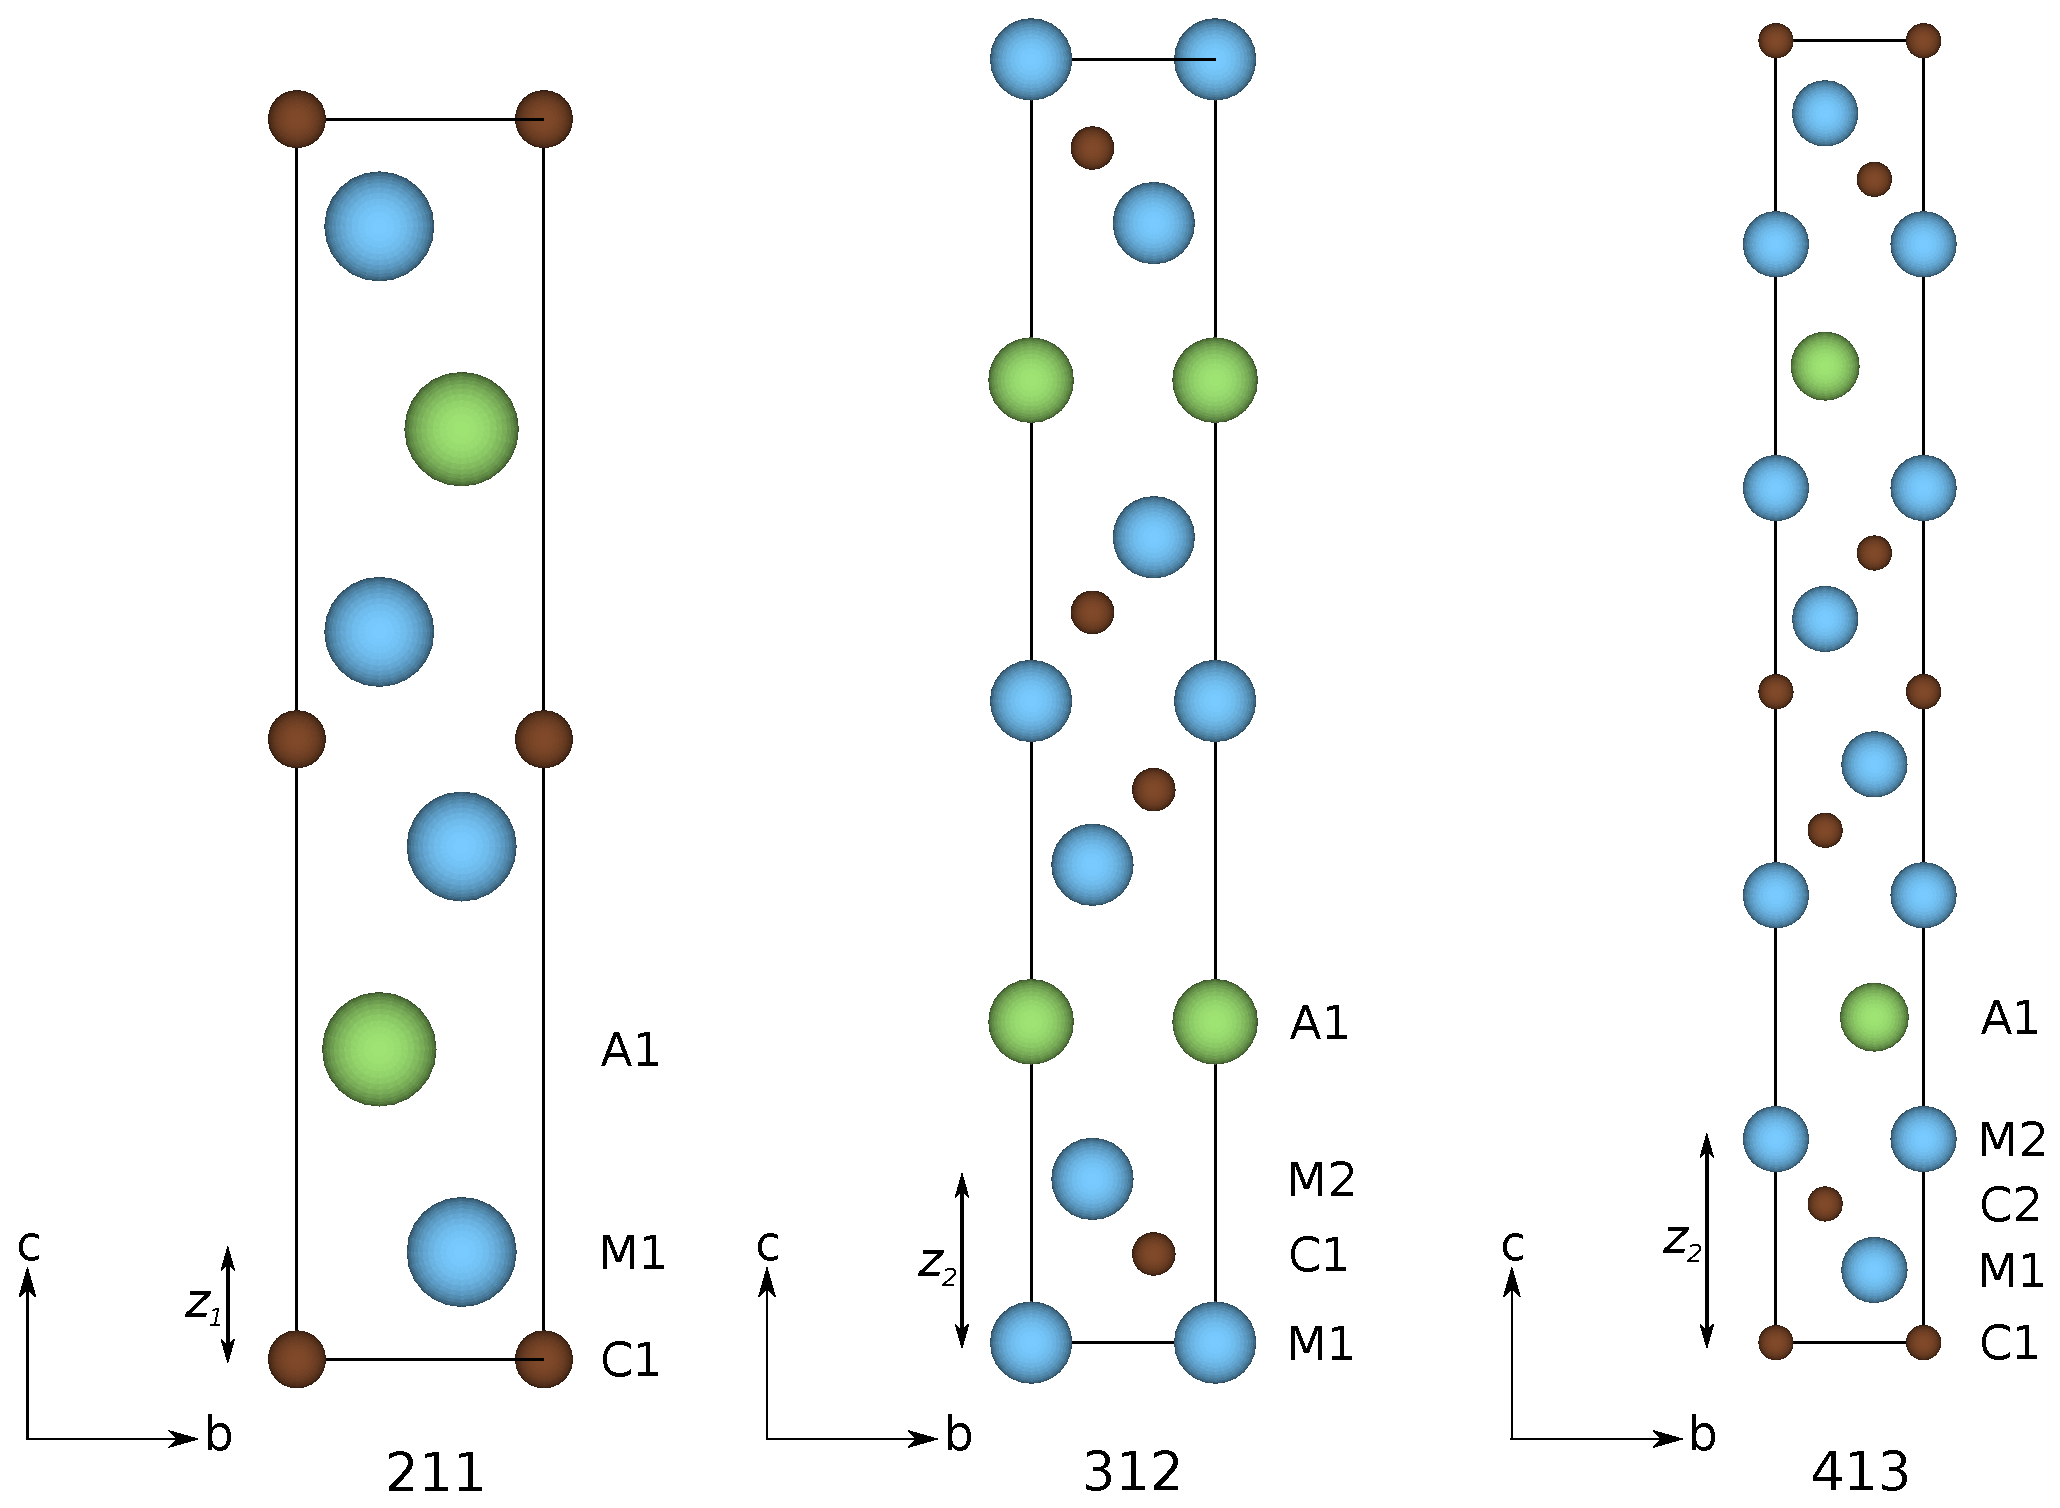
\includegraphics[width=\textwidth]{MAX_unit_cells}
\caption{The unit cells of the first three possible MAX phases.\label{fig:MAX_unit_cells}}
\end{figure}




\begin{figure}
\centering
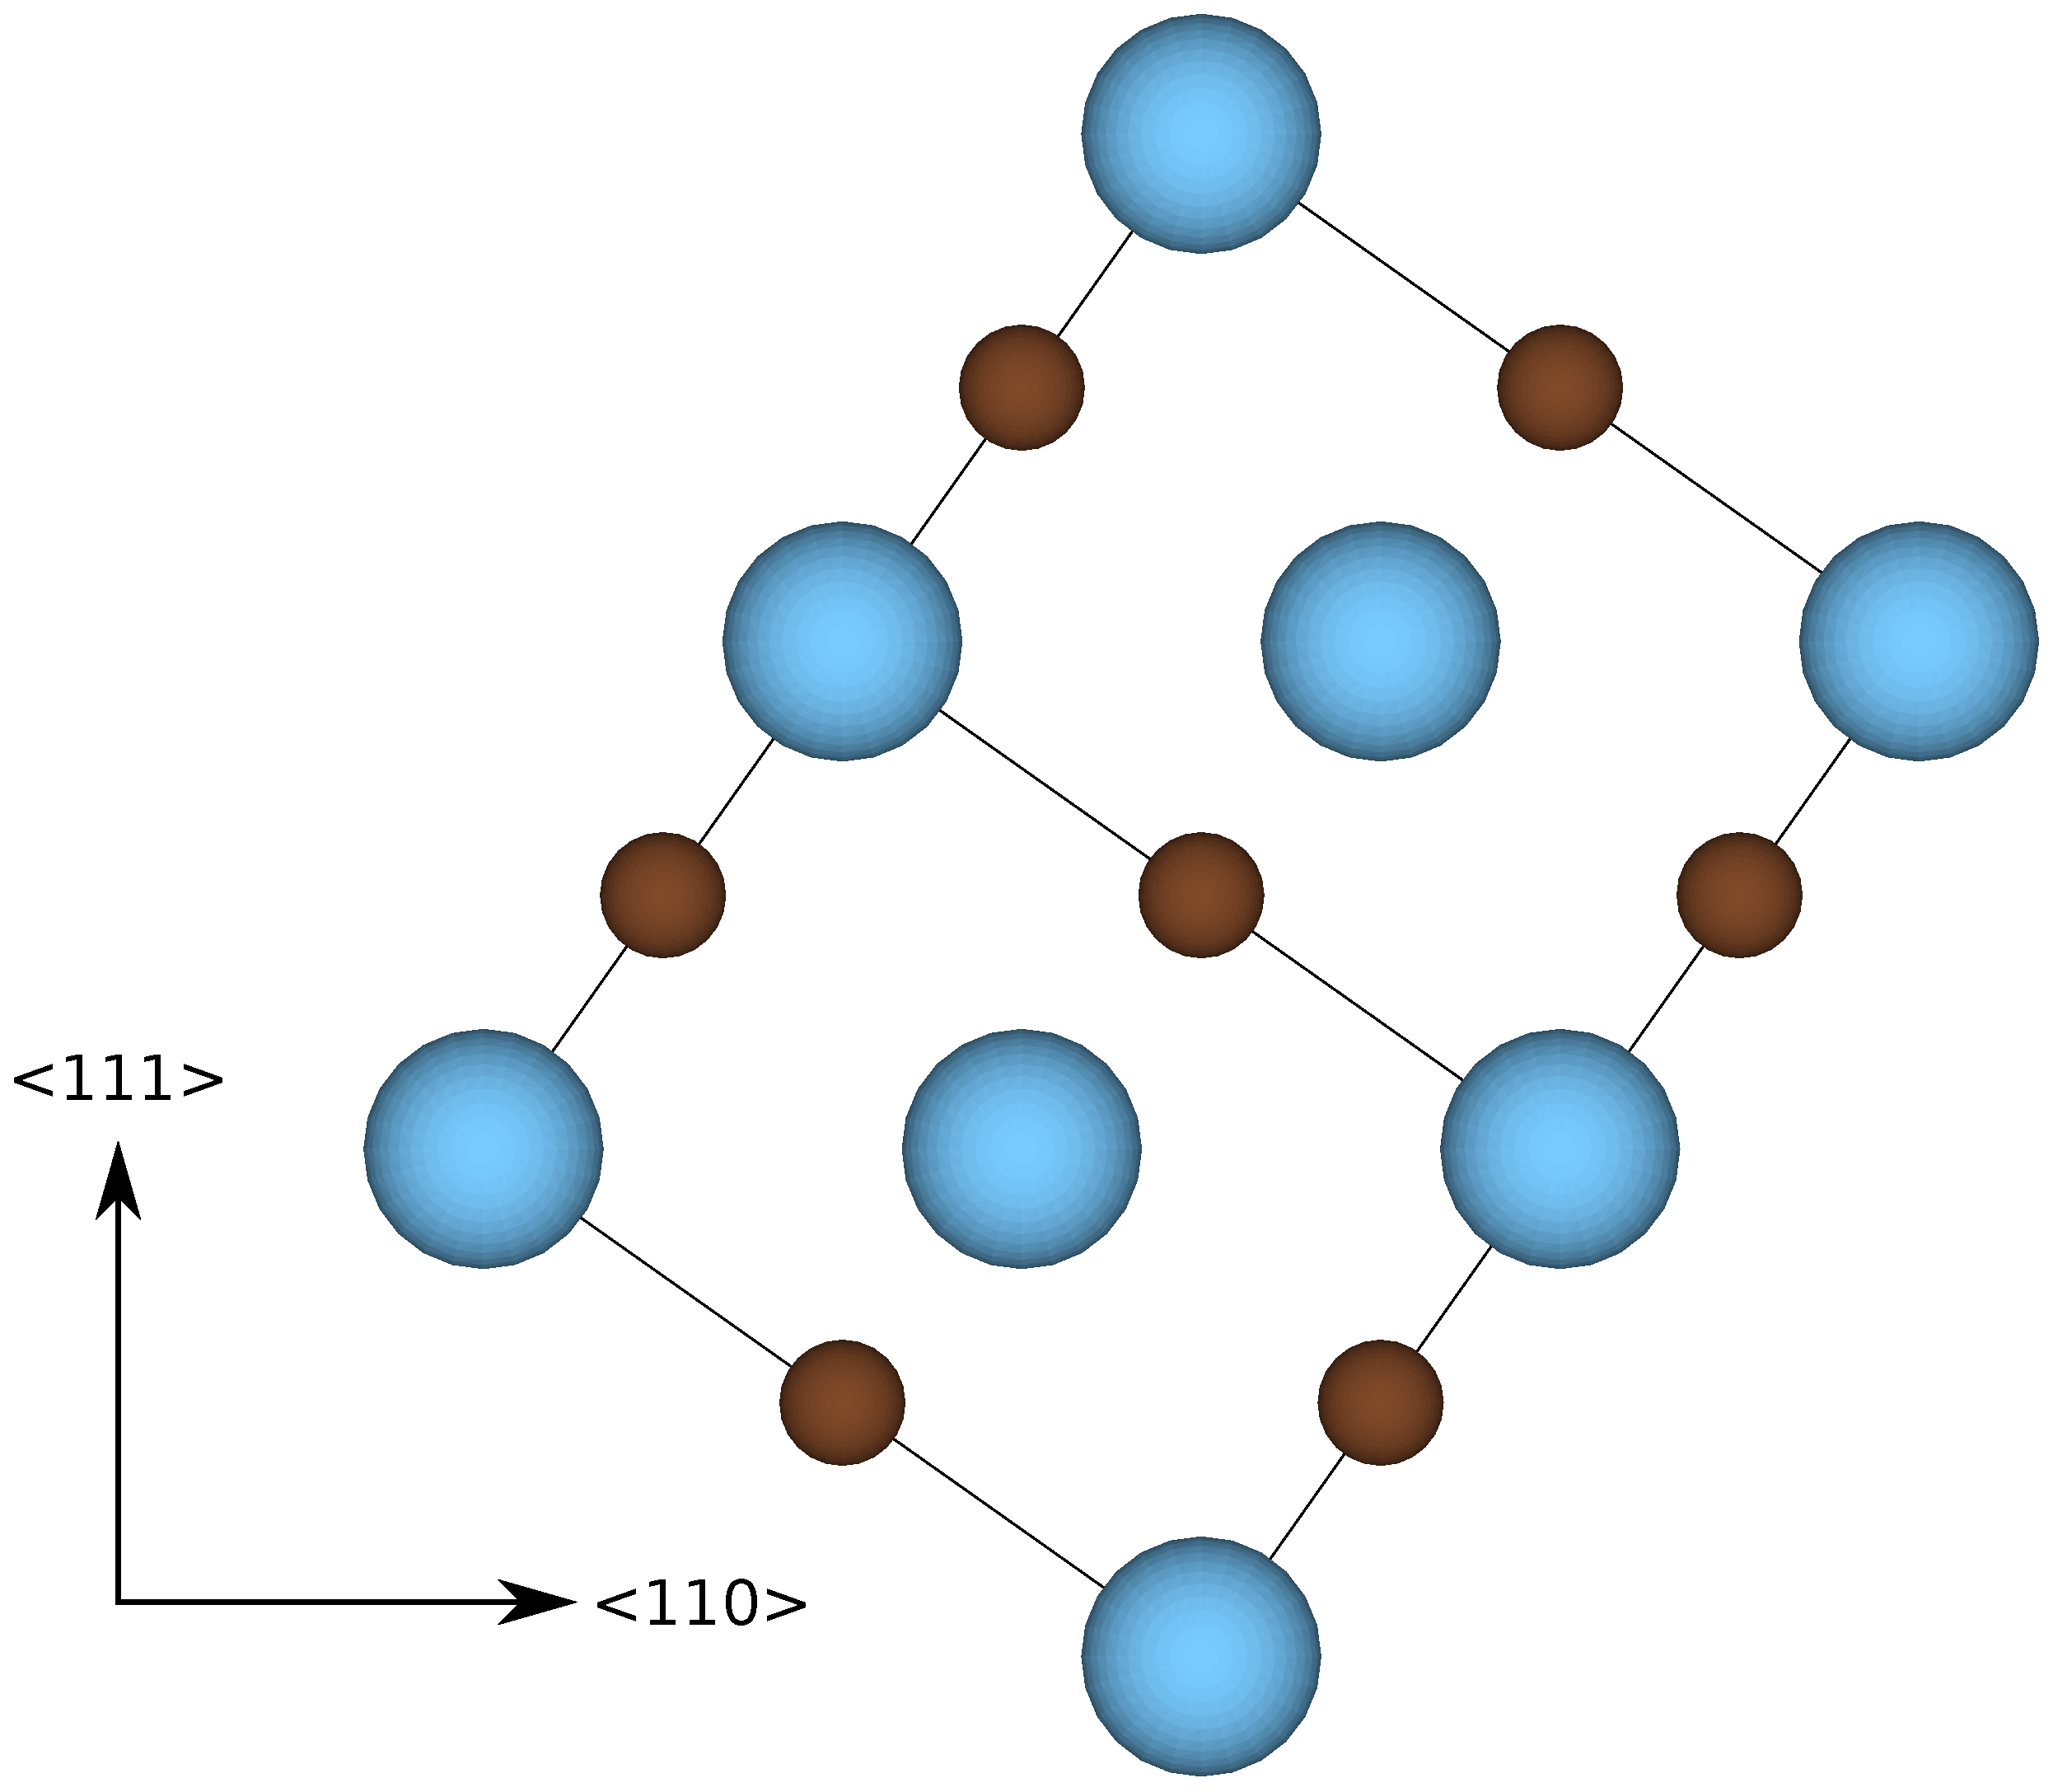
\includegraphics[width=0.5\textwidth]{TiC_111}
\caption{The unit cell of \ce{TiC}, which has the rocksalt structure, oriented to show the \{111\} planes which are equivalent to the MX layers of the MAX structure shown in \ref{fig:MAX_unit_cells}. \label{fig:TiC_111}}
\end{figure}


The description of complex crystals is often elucidated by geometrically salient features, for example is quasicrystals and quasicrystal-approximants structures are often described in terms of clusters of atoms that appear to pack together and fill space; the clusters may or may not have physical significance, for example stable clusters of up to 55 atoms of \ce{Ni}-\ce{Al} are stable on surfaces and so is clearly stabilised and physcically significant, but geometric descriptions of clusters can be made of simple materials like fcc aluminium \cite{Steurer2006}. Care must be taken therefore not to ascribe undue significance to purely geometric features, but the description of the MAX crystal structure as layers is no simply elucidating but can be justified.

The bonding in MAX phases has been shown, by density functional theory (DFT) calculations to be a combination of metallic, covalent and ionic bonding but with covalent bonding predominant in the MX layer and metallic bonding in MA layers but with large variations in structural and mechanical properties observed to depend on changes in the nature of this heterogeneous bonding character \cite{Radovic2013,Sun2011}. Notably the extreme (for MAX phases) properties of \ce{Ti2SC} are ascribed to the unusual strong bonding between \ce{Ti} and \ce{S} in addition to the strong bonding between \ce{Ti} and \ce{C} in contrast with most other MAX. This unusual bonding is taken to underlie the high elastic constants, $E =$~\SI{316}{\giga\pascal} the highest of any 211 MAX phase, and hardness of \SI{8}{\giga\pascal}, very nearly the highest of any bulk MAX phase \cite{Feng2010, Sun2011}.

\subsection{Deformation in MAX phases}

Deformation in \ce{Ti3SiC2} has been widely studied, particularly by Barsoum \cite{Farber1998,Barsoum1999,Farber1999,Barsoum1999dislocs_kinkbands,Barsoum2001}, and was found to readily occur by the glide of dislocations. Room temperature deformation was shown to increase the density of perfect basal dislocations with a Burgers vector equal to the lattice parameter $a$, or $b =$~<11\={2}0>. 

Using heavily textured bulk samples of \ce{Ti3SiC2} the critical resolved shear stress of \ce{Ti3SiC2} was estimated by compression test. A smaple with the basal planes of the sample oriented at approximately \SI{65}{\degree} to the compression axis and a yield stress of \SI{200}{\mega\pascal} was measured. Schmid's law is 

\begin{equation}
\tau_y = \sigma_y \cos{\phi} \cos{\lambda}
\end{equation}

where $\tau_y$ is the shear yield stress on the slip plane in question, $\sigma_y$ is the uniaxial yield stress\ $\phi$ is the angle between the slip plane normal and the loading axis, and $\lambda$ is the angle between the slip direction and the loading axis. The $\phi$ must be \SI{25}{\degree} ($=\SI{90}{\degree} - \SI{65}{\degree}$) but $\lambda$ is not known but if taken to be the maximum possible value, given $\phi=\SI{25}{\degree}$, of \SI{115}{\degree} then $\tau_y = \SI{77}{\mega\pascal}$, providing an upper bound \cite{Humphrey2012}. While this is higher than the estimate made by the original authors \cite{Barsoum1999}, \citet{Humphrey2012} points out that this is likely an overestimate due to the variation in Schmid factor across the sample and load redistribution between soft and hard grains but in any case is very low for a ceramic and approaches the flow stresses of pure cubic close-packed metals.


%%%%%%%%%%%%%%%%%%%%%%%%%%%%%%%%%%%%%%%%%%%%%%%%%%%%%%%%%%%%%%%%%%
%
%
%
%
%
%
% Figure about compression test here?
%
%
%
%
%
%
%%%%%%%%%%%%%%%%%%%%%%%%%%%%%%%%%%%%%%%%%%%%%%%%%%%%%%%%%%%%%%%

Attempts to relate the electronic structure to plasticity have been made, but even recently such studies have tended to find structural, physical and elastic properties of ``complex'' materials and then infer the relative ductility on the basis of these properties. For example some ternary metal nitrides with chemistry obeying \ce{Ti_xM_{1-x}N} are of interest as wear resistant coatings and increased toughness is very desirable and studies have predicted that the use of \ce{Mo} or \ce{W} as alloying additions significantly improve the toughening, indeed the effect has been dubbed ``\emph{supertoughening}'' \cite{Sangiovanni2010,Sangiovanni2011}. The studies uses \emph{ab initio} calculations to find the elastic response of the alloyed crystal to an applied strain. The study finds a number of interesting things including the development of a layered electronic structure and trends for elastic properties, particularly the Pugh ratio, $B/G$, with the valence electron concentration. The authors speculate about selective local responses to stress, though with little concrete basis for doing so since the elastic constants were calculated from the energy changes under various applied \emph{uniform} shear strains.

However the conclusions drawn from these elastic simulations about plasticity can be, at best, qualitative. In fact these studies employ on arguments of easily broken bonds since ``during dislocation motion bonds are broken and reformed and, obviously, dislocation glide will occur more easily in planes normal to those containing weaker bonds'' \cite{Sangiovanni2011} without further justification. Clearly this is not a mechanistic explanation for the effect of chemical bonding on plasticity relying as it does on dated and empirical ratios of elastic constants.

A study on MAX phases \cite{Music2007ductility} with the chemistry \ce{M2AlC} (M = Ti, V, Cr) used the more recent ductility criteria, namely Zhou-Carlsson-Thomson \cite{Zhou1994} and Rice \cite{Rice1992} which are discussed in detail in \autoref{subsec:ductility_criteria}, here there is some recognition that the lattice resistance of a single dislocation, which is after all the limiting factor on ductility in most ceramics, is not simply dependent on bulk elastic constants and instead calculate ductility criteria based on stacking fault energies and surface energies, which necessitates choosing which plane to fault or cleave. In the MAX phases there are two natural choices for a 211 MAX phase, between the M atom and the A atom or between the M atom and the X atom. Once again however there is no mechanistic link between these properties and the proposed good ductility. 

























\FloatBarrier
\section{Ionic crystals}
\FloatBarrier
\label{sec:ionic_crystals}


The Peierls model is based on the assumption that energy changes can be largely approximated on elastic energy changes as a dislocation moves through a crystal lattice, but many materials do not fit this assumption well. Ionic solids are an obvious and large class of materials that fall into this category.

Though the energy of ionic crystals is relatively easily calculated for a perfect crystal, via a Madelung or Ewald summation \cite{madelung1918,Ewald1921}, these rest on assumption of symmetry that are broken by the introduction of a defect.

The rocksalt structure is particularly common in ionic solids and phases of this structure have been widely studied in terms of their plasticity. The slip direction is usually <110> and the active slip planes are \{001\} and \{1\={1}0\}, and sometimes \{1\={1}1\}. For edge dislocations the last would expose charged surfaces of atoms at free surfaces so despite being the closest packed plane it is not commonly seen \cite{Haasen1985}.



























































